\documentclass[12pt,a4paper,twoside]{report}
\usepackage[italian]{babel}
\usepackage{newlfont}
\usepackage{color}
\textwidth=450pt\oddsidemargin=0pt

% INIZIO HEADER INSERITI DA ME, DA CUI HO TOLTO GLI HEADER CHE SI RIPETONO

%\documentclass[12pt,a4paper]{article}
%\usepackage[utf8]{inputenc}
\usepackage{titling}
\usepackage[backend=bibtex,
			style=numeric,
			sorting=none
			]{biblatex}
\addbibresource{bibliography.bib} %Import the bibliography file
%\setlength{\droptitle}{-2cm}% change title position
\usepackage{amsmath}
%\usepackage{amsfonts}
\usepackage{amssymb}
%\usepackage[T1]{fontenc}
\usepackage{tablefootnote}
\usepackage{multirow}
\usepackage{array}
\newcolumntype{P}[1]{>{\centering\arraybackslash}p{#1}}
\newcolumntype{M}[1]{>{\centering\arraybackslash}m{#1}}
\usepackage{graphicx}
\usepackage[version=4]{mhchem}
%\usepackage{siunitx}
\usepackage{float}
\usepackage[top=1.7in,left=1in,right=1in]{geometry}
%\usepackage{listings}
%\usepackage{circuitikz}
\usepackage{subcaption}
\usepackage{tabularx}
%\renewcommand{\lstlistingname}{Code}
%\renewcommand{\lstlistlistingname}{List of Code}
%\lstdefinestyle{chstyle}{
	%	backgroundcolor=\color{gray!12},
	%	basicstyle=\ttfamily\small,
	%	commentstyle=\color{green!60!black},
	%	keywordstyle=\color{magenta},
	%	stringstyle=\color{blue!50!red},
	%	showstringspaces=false,
	%	%captionpos=b,
	%	numbers=left,
	%	numberstyle=\footnotesize\color{gray},
	%	numbersep=10pt,
	%	%stepnumber=2,
	%	tabsize=2,
	%	frame=L,
	%	framerule=1pt,
	%	rulecolor=\color{red},
	%	breaklines=true,
	%	inputpath=code
	%}
%\renewmenumacro{\directory}{pathswithfolder} % default: path
%\renewmenumacro{\keys}{shadowedroundedkeys} % default: roundedkeys
\setlength{\arrayrulewidth}{0.9pt}
\renewcommand{\arraystretch}{1.3}
\usepackage{mathcomp}

%\usepackage{fontspec}
%\setmainfont{Calibri}

\usepackage{fancyhdr}
\pagestyle{fancy}
%\renewcommand{\chaptermark}[1]{\markboth{\MakeUppercase{\chaptername\ \thechapter.\ #1}}{}}
\renewcommand{\chaptermark}[1]{\markboth{\MakeUppercase{CAP.\ \thechapter\ --\ #1}}{}}
\setlength{\headwidth}{13cm}
\fancyhead{} % clear all header fields
\fancyhead[LO]{\footnotesize \textsl{\rightmark}}
\fancyhead[RE]{\footnotesize \textsl{\leftmark}}
\fancyhead[LE,RO]{\footnotesize \thepage}
\fancyfoot{} % clear all footer fields
\renewcommand{\headrulewidth}{0.3pt}

% è già di default interlinea singola
\usepackage{setspace}

\newsavebox{\largestimage}

%\usepackage[font=it]{caption}
%\usepackage{indentfirst}
%\interfootnotelinepenalty=\@M

\usepackage{hyperref}
\hypersetup{
	colorlinks,
	citecolor=black,
	filecolor=black,
	linkcolor=black,
	urlcolor=black
}

% FINE HEADER INSERITI DA ME

\begin{document}
	\pagenumbering{roman}
	\begin{titlepage}
		\begin{center}
			{{\Large{\textsc{Alma Mater Studiorum $\cdot$ Universit\`a di Bologna}}}} 
			\rule[0.1cm]{15.8cm}{0.1mm}
			\rule[0.5cm]{15.8cm}{0.6mm}
			\\\vspace{3mm}
			
			{\small{\bf Scuola di Scienze \\ 
					Dipartimento di Fisica e Astronomia\\
					Corso di Laurea in Fisica}}
			
		\end{center}
		
		\vspace{23mm}
		
		\begin{center}\textcolor{red}{
				%
				% INSERIRE IL TITOLO DELLA TESI
				%
				{\LARGE{\bf TITOLO TESI}}\\
		}\end{center}
		
		\vspace{50mm} \par \noindent
		
		\begin{minipage}[t]{0.47\textwidth}
			%
			% INSERIRE IL NOME DEL RELATORE CON IL RELATIVO TITOLO DI DOTTORE O PROFESSORE
			%
			{\large{\bf Relatore: \vspace{2mm}\\\textcolor{red}{
						Prof./Dott. Nome Cognome}\\\\
					%
					% INSERIRE IL NOME DEL CORRELATORE CON IL RELATIVO TITOLO DI DOTTORE O PROFESSORE
					%
					% SE NON AVETE UN CORRELATORE CANCELLATE LE PROSSIME 3 RIGHE
					%
					\textcolor{red}{
						\bf Correlatore: (eventuale)
						\vspace{2mm}\\
						Prof./Dott. Nome Cognome\\\\}}}
		\end{minipage}
		%
		\hfill
		%
		\begin{minipage}[t]{0.47\textwidth}\raggedleft {
				{\large{\bf Presentata da:
						\vspace{2mm}\\
						Simone Pasquini}}}
		\end{minipage}
		
		\vspace{40mm}
		
		\begin{center}
			Anno Accademico { 2023/2024}
		\end{center}
		
	\end{titlepage}
	\newpage
	\newgeometry{top=4cm,bottom=4cm,left=4cm,right=4cm}
	\doublespacing % Also singlespacing, onehalfspacing 
	\chapter*{Sommario (TBD)}
		Questo è l'inizio del sommario.
	\newpage
	\tableofcontents
	\newpage
	\addcontentsline{toc}{chapter}{Introduzione (TBD)}
	\chapter*{Introduzione (TBD)}
		Questo è l'inizio dell'introduzione. metodo del SSN (sistema già attivo nella sanità+Questo percorso ha portato alla marcatura CE del centro e nel 2017 l'adroterapia è stata inserita nei Livelli Essenziali di Assistenza.
		
		 statale).https://scienzapertutti.infn.it/4-adroterapia-dalla-fisica-alla-terapia
	\newpage
	
	\pagenumbering{arabic}
	
	\chapter{Terapie oncologiche e radiazioni ionizzanti}
	\section{Incidenza tumorale nel mondo}\label{sec:1.1}
	Tra le principali cause di morte della popolazione mondiale è possibile annoverare le neoplasie (o tumori) ovvero neoformazioni che, a causa di mutazioni genetiche che sfuggono ai meccanismi di controllo della proliferazione cellulare, iniziano a crescere, senza alcuna finalità, in maniera incontrollata e scoordinata rispetto al tessuto sano. \`E possibile distinguere due tipi di neoplasie: benigne e maligne. Mentre le prime si limitano alla sede di origine, le seconde generano metastasi, un processo in cui le cellule neoplastiche si spostano dalla sede originaria e danno origine a masse anomale che invadono altri tessuti dell'organismo, ostacolandone le funzioni vitali. In questo ultimo caso si parla di tumore maligno o cancro.
	
	Attualmente, è possibile prevenire fino al $50\%$ di tumori evitando fattori di rischio e implementando strategie di prevenzione già esistenti (cita
	%https://www.who.int/news-room/fact-sheets/detail/c+ancer
	), anche se ciò dipende dalla tempestività delle diagnosi, dalla tipologia delle cure e dal tipo di tumore. Si stima che nei Paesi industrializzati,\footnote{Si fa riferimento ai Paesi OCSE (Organizzazione per la Cooperazione e lo Sviluppo Economico).} nel $2021$, il cancro è la seconda causa di morte (causando il $21\%$ dei decessi totali), preceduto dalle malattie cardiovascolari (cita %https://www.oecd-ilibrary.org/docserver/7a7afb35-en.pdf?expires=1709230714&id=id&accname=guest&checksum=FBEABF3EDA6F2040465BB27356B8D68B
	). Sebbene il tasso di mortalità sia sceso sin dal $2000$, a livello mondiale il numero di casi diagnosticati di cancro (nel $2022$) attesta a quasi $20.0$ milioni\footnote{Negli ultimi dieci anni il numero di casi di tumore è aumentato di anno in anno, soprattutto a causa dell'invecchiamento progressivo della popolazione (cita
	%https://www.iss.it/-/tumori-in-aumento-le-diagnosi-in-europa-anche-per-effetto-dell-invecchiamento-demografico
	), ma nel biennio $2020$-$2021$ il trend è cambiato a causa della pandemia di COVID-$19$, che ha precluso l'accesso a screening oncologici (nel periodo gennaio--ottobre $2020$ vi è stato un calo del $37.3\%$ di test diagnostici rispetto al periodo pre-pandemico) (cita
	%https://www.ncbi.nlm.nih.gov/pmc/articles/PMC9807424/
	). Ciò potrebbe rivelarsi fatale nel medio-lungo termine causando un aumento dei tassi di incidenza e mortalità (cita
	%https://doi.org/10.1787/ae3016b9-en
	).} (pari al $2.5\tcperthousand$ della popolazione totale (citare %https://data.unicef.org/resources/data_explorer/unicef_f/?ag=UNICEF&df=GLOBAL_DATAFLOW&ver=1.0&dq=WORLD.DM_POP_TOT.&startPeriod=2022&endPeriod=2022
	)), di cui il $48.8\%$ hanno portato alla morte del paziente (citare
	%https://gco.iarc.who.int/en
	). Inoltre, i tassi di mortalità dovuti alle patologie tumorali sono strettamente dipendenti dall'indice di sviluppo dei Paesi (ISU), infatti da un tasso di mortalità del $39.2\%$ dei Paesi con ISU molto alto, si sale sino al $67.1\%$ dei Paesi con basso ISU (cita
	%https://gco.iarc.who.int/today/en/dataviz/bars?mode=population&key=total&group_populations=0&types=0_1&sort_by=value1&populations=900_981_982_983_984&multiple_populations=1&values_position=out&cancers_h=39&include_nmsc=1&age_end=17
	).
	
	Altri fattori rendono i tassi di incidenza e mortalità per patologie tumorali ulteriormente disuniformi, quali il sesso e l'età. A livello globale, l'incidenza di cancro negli uomini è più alta rispetto a quella delle donne dell'$8.0\%$ (cita
	%https://gco.iarc.who.int/media/globocan/factsheets/cancers/39-all-cancers-fact-sheet.pdf
	), dovuta anche al fatto che i primi si espongono maggiormente a fattori di rischio quali fumo e consumo di alcol. Inoltre, il $58\%$ di tumori viene diagnosticato nelle persone con più di 65 anni (cita
	%https://www.cdc.gov/cancer/uscs/about/data-briefs/no29-USCS-highlights-2019-incidence.htm
	).
	
	Sebbene i dati sopra citati testimonino la gravità delle patologie oncologiche, è indubbio che il progresso della scienza degli ultimi anni abbia permesso un notevole sviluppo nell'efficacia dei trattamenti oncologici: nel decennio $2010$--$2020$, il numero di persone che sopravvive dopo una diagnosi di cancro aumenta approssimativamente del $3\%$ in Paesi come l'Italia, gli Stati Uniti d'America, il Regno Unito e la Svizzera (cita
	%https://www.ncbi.nlm.nih.gov/pmc/articles/PMC5807846/pdf/12885_2018_Article_4053.pdf
	).
	
	\section{Terapie oncologiche}\label{sec:1.2}
	Il trattamento di un tumore avviene in molti modi differenti e varia in base al tipo di cancro, il suo stadio di avanzamento e dagli obiettivi che si intendono raggiungere al termine dei trattamenti. Oggigiorno, le terapie oncologiche si distinguono in locali (o regionali) e generali (o sistemiche), in base all'estensione del tumore che colpisce il paziente. Al primo gruppo appartengono terapie come la chirurgia, la radioterapia e l'adroterapia, mentre al secondo afferiscono la chemioterapia e l'immunoterapia. Tali tecniche, proprio per la loro diversità, sono spesso utilizzate in maniera complementare per aumentare l'efficacia dei trattamenti clinici. Per pianificare il trattamento più adeguato al fronte di una certa patologia oncologica, si introduce il concetto di stadiazione, che è un modo di descrivere in maniera schematica, rigorosa e standardizzata la grandezza di un tumore e la sua diffusione al di fuori della sede originale (cita
	%https://www.airc.it/cancro/affronta-la-malattia/la-fase-della-diagnosi/stadiazione
	). Le informazioni tipiche della stadiazione includono la collocazione del tumore, la sua estensione e se si è diffuso in parti del corpo differenti. Infatti, come già accennato, le cellule tumorali si moltiplicano in modo incontrollato andando a occupare (per mezzo del sistema linfatico o sanguigno) organi e tessuti distanti dalla sede di sviluppo originaria, attraverso un fenomeno chiamato metastatizzazione. Chiaramente, ciascuna terapia possiede effetti collaterali correlati all'azione distruttiva che si impiega per debellare la malattia oncologica.
	
	Se il tumore ha raggiunto un'estensione tale da formare metastasi, si scelgono trattamenti sistemici in modo che si possa debellare o, quantomeno, contenere la malattia oncologica. La chemioterapia consiste nella somministrazione di uno o più farmaci citotossici (o antiblastici) capaci di aggredire le cellule cancerose (cita
	%https://www.aimac.it/libretti-tumore/chemioterapia/che-cos-e-la-chemioterapia
	), mentre nell'immunoterapia si tenta di istruire il sistema immunitario affinché riconosca ed elimini le cellule malate che, in assenza di trattamento clinico, appaiono "nascoste" al sistema immunitario stesso.
	
	Qualora il tumore fosse localizzato, ben raggiungibile dall'esterno e sufficientemente lontano da organi vitali, si ricorre a operazioni chirurgiche, con le quali si asporta la massa tumorale dal corpo del paziente. Prima o dopo l'operazione chirurgica, si procede con tecniche radioterapiche, adroterapiche o chemioterapiche in base alle necessità. Ad esempio, nella radioterapia neoadiuvante il trattamento radioterapico viene effettuato prima dell'intervento chirurgico, mentre nella radiochemioterapia concomitante si eseguono sessioni di chemioterapia e radioterapia a seguito dell'operazione chirurgica (cita
	%https://www.aimac.it/libretti-tumore//perche-si-attua-la-radioterapia
	). In generale, la commistione di suddette tecniche consente di rimuovere tracce di cellule tumorali, evitandone eventuali proliferazioni successive.
	
	Nel caso in la massa tumorale non sia rimovibile attraverso un'operazione chirurgica a causa della sua localizzazione anatomica (è il caso di neoplasie legate a organi la cui rimozione sarebbe troppo invalidante per il paziente (cita
	%https://web.infn.it/foot/
	)), si preferisce ricorrere alla radioterapia e all'adroterapia, ove quest'ultima è una forma avanzata di radioterapia. Pur non essendo invasive come la chirurgia, tali tecniche permettono di danneggiare specifici tessuti biologici malati utilizzando radiazione ionizzante, composta da fasci di fotoni ed elettroni in radioterapia e da particelle adroniche (come protoni, neutroni e ioni) in adroterapia (si veda \hyperref[fig:simulation]{Fig. 1.1}). In particolare, lo scopo di entrambi i trattamenti è quello di depositare una quantità di energia (detta "dose") capace di provocare un danno biologico tale da inibire la crescita del tumore con effetti collaterali minimi (cita
	%rivista asimmetrie, DOI 10.23801/asimmetrie.2023.35.03
	). Sebbene sembrino molto simili, la radioterapia e l'adroterapia presentano caratteristiche fisiche e radiobiologiche molto differenti, i cui dettagli verranno evidenziati nel prosieguo. Mentre un fascio radioterapico rilascia la dose in una regione piuttosto ampia, aumentando il rischio di distruggere cellule sane situate prima e dopo il tumore, le particelle adroniche irradiano una grande quantità di energia in uno spazio molto limitato, attraverso il caratteristico picco di Bragg. Pertanto, visto che l'adroterapia permette di definire in modo molto più preciso la regione da irradiare (cita
	%https://web.infn.it/foot/
	), il suo obiettivo non è solo quello di distruggere più efficacemente porzioni di cellule tumorali, ma anche quello di minimizzare i danni a carico dei tessuti sani circostanti (cita
	%https://fondazionecnao.it/adroterapia/cos-e-l-adroterapia
	), al fine di migliorare la qualità della vita del paziente.
	
	\begin{figure}[H]
		\centering
		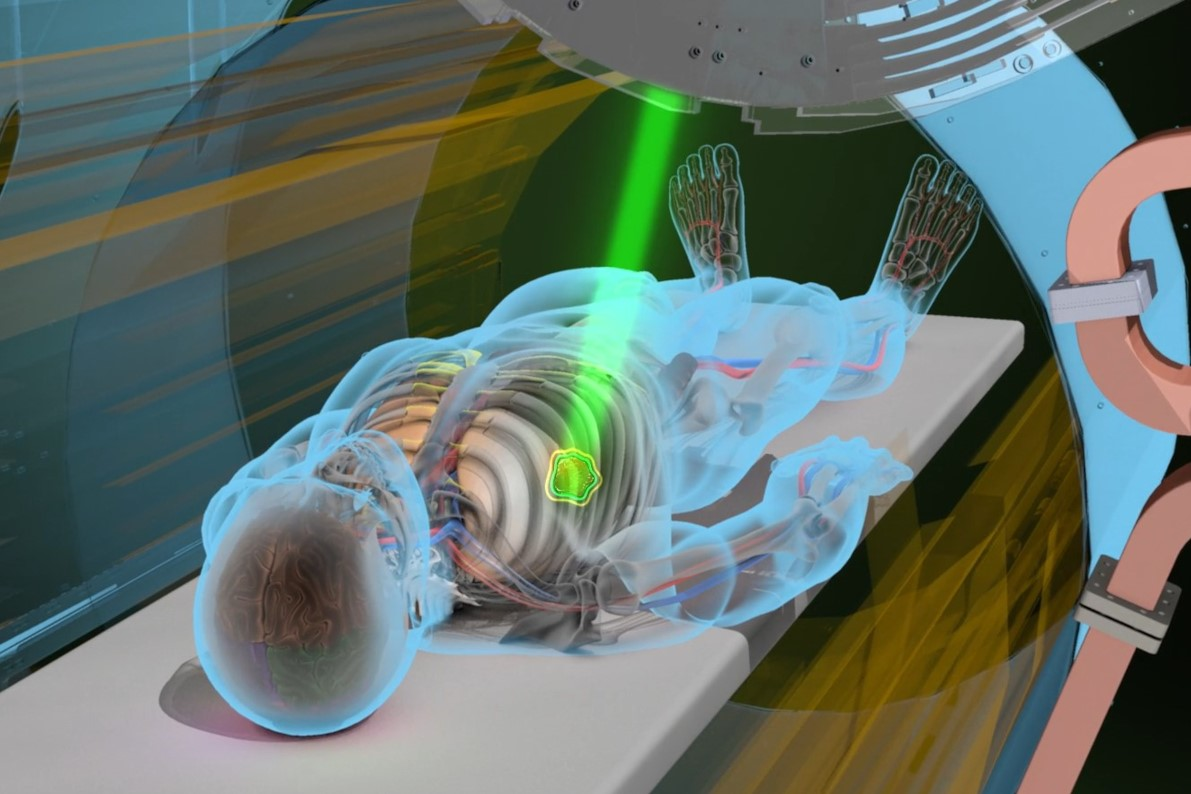
\includegraphics[width=0.9\linewidth]{images/simulation.jpg}
		\caption{Simulazione di un irraggiamento radioterapico o adroterapico sul corpo di un paziente (cita
			%https://www.youtube.com/watch?v=Uu261OEf3Pg
			).}
		\label{fig:simulation}
	\end{figure}
	
	Sebbene l'adroterapia sia complessivamente più efficace rispetto alla radioterapia nella distruzione di cellule tumorali e nella salvaguardia dei tessuti sani, è un trattamento relativamente recente (si veda \hyperref[storia_adroterapia]{Sez. ??}) che ha bisogno, tra le varie e complesse strutture, di acceleratori di particelle; ciò rende l'adroterapia meno sviluppata e più costosa della radioterapia. Inoltre, oggi non esiste una teoria analitica che sia in grado di spiegare i processi nucleari che intercorrono tra le particelle adroniche e i nuclei del corpo umano (cita
	%FOOT CDR
	), quindi, prima di poter applicare trattamenti medici efficaci e sicuri, si rendono necessarie numerosissime misure sperimentali (una buona parte delle quali sono tuttora fornite dall'esperimento FOOT) in grado di colmare tali lacune (cita
	%https://web.infn.it/foot/
	). Per questo motivo, il settore di ricerca adroterapico è molto attivo e coinvolge un crogiolo culturale di fisici, medici, biologi che studiano gli effetti della frammentazione nucleare sulle cellule umane, analizzabili solo mediante un approccio interdisciplinare.
	
	L'adroterapia, però, non appartiene esclusivamente all'ambito della sperimentazione, ma costituisce una realtà interazionale nella cura dei tumori a tutti gli effetti. Infatti, alla fine del $2023$ quasi $410000$ pazienti hanno effettuato trattamenti adroterapici a livello globale (di cui $350000$ con protoni, $56000$ con ioni carbonio e $3500$ con elio, pioni e altre particelle), un numero tre volte maggiore di quello emerso a fine $2014$ (cita
	%https://ptcog.site/
	). Pur essendo tali numeri incoraggianti, è necessario continuare a investire risorse nella ricerca in modo che esperimenti della caratura di FOOT possano rendere l'adroterapia un trattamento più diffuso e accessibile a tutti.
	
	\section{Storia della radioterapia}
	La storia della radioterapia inizia nel novembre del $1895$ con un episodio di serendipità, il cui protagonista è il fisico tedesco Wilhelm C. von Röntgen ($1845$--$1923$), scopritore dei raggi X. Durante lo studio dei raggi catodici prodotti da un tubo di Crookes, Röntgen si accorse che della radiazione sconosciuta (denominata da lui stesso "X", poiché incognita sino ad allora) oltrepassava la lastra di vetro che ricopre lo strumento. Röntgen comprese sin da allora le grandi potenzialità dei neonati raggi X, utilizzabili per proiettare su uno schermo il materiale che attraversano delineandone le specificità. Fu proprio il fisico a effettuare la prima radiografia alla mano di sua moglie (\hyperref[fig:rongten]{Fig. 1.2}), esponendo tuttavia quest'ultima a non pochi rischi, essendo i raggi X un tipo di radiazione ionizzante.\footnote{Una radiazione si dice ionizzante quando ha energia sufficiente a liberare gli elettroni legati agli atomi della materia in cui penetra. Per questo motivo la radiazione ionizzante è capace di provocare danni biologici ai tessuti del corpo umano.} Le immediate applicazioni della scoperta di Röntgen in campo medico gli valsero il premio Nobel per la fisica nel $1901$(cita
	%https://www.nobelprize.org/prizes/physics/1901/rontgen/facts/
	).
	
	\begin{figure}[H]
		\centering
		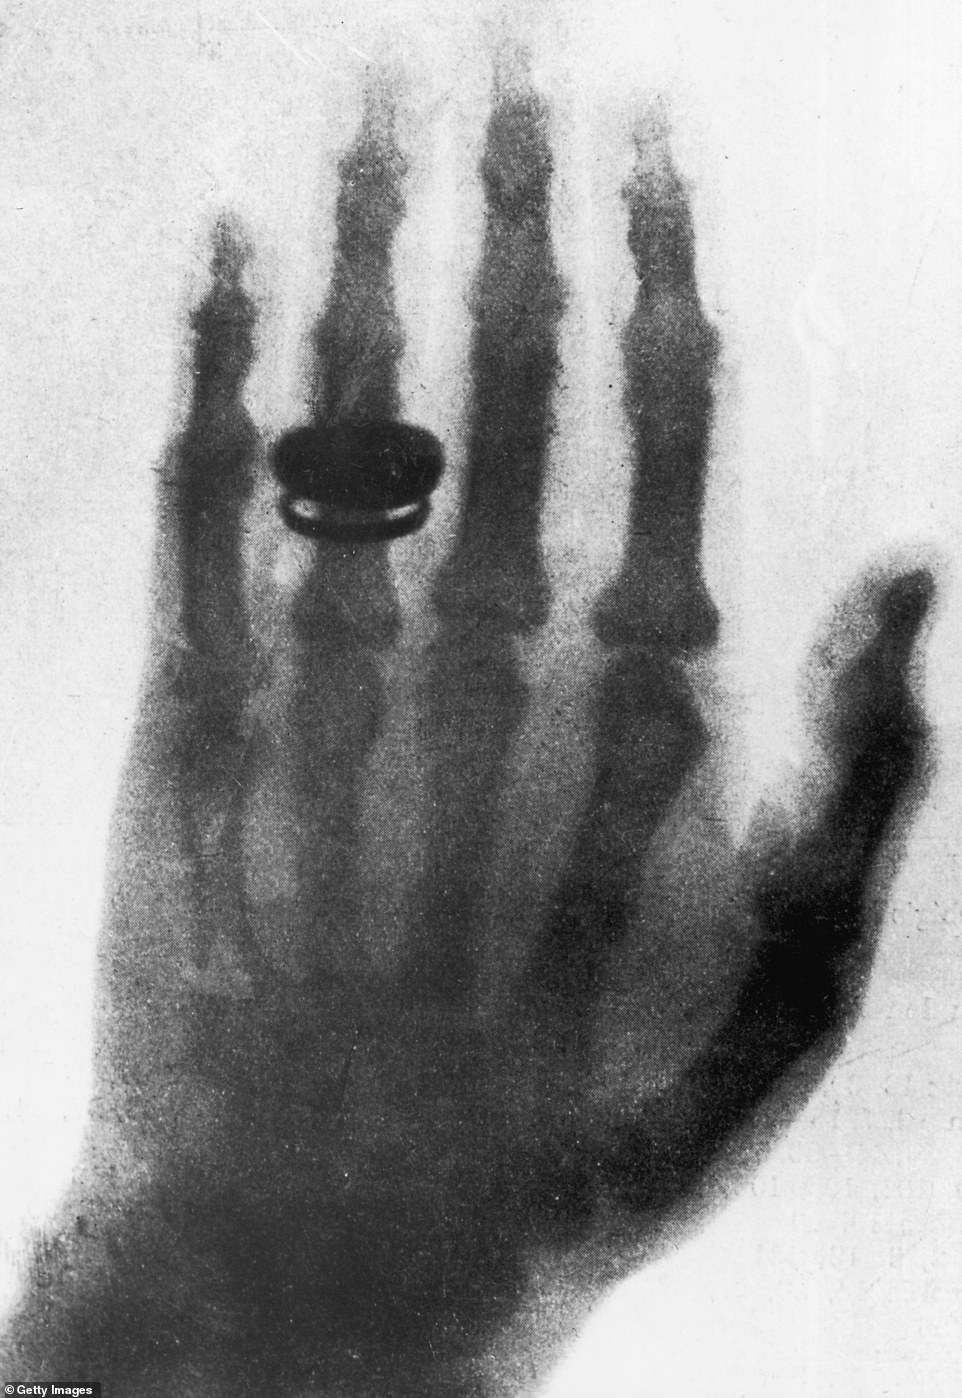
\includegraphics[width=0.5\linewidth]{images/rongten.jpg}
		\caption{La prima lastra a raggi X della mano di Anna Bertha Ludwig, moglie di Ron, dopo 15 minuti di esposizione (cita
			%https://www.dailymail.co.uk/news/article-6491287/Roentgens-human-X-ray-wifes-hand-1895.html
			).}
		\label{fig:rongten}
	\end{figure}
	
	Solamente un anno dopo la scoperta di Röntgen, Antoine H. Becquerel ($1852$--$1908$), studiando la fosforescenza dei sali di uranio, notò che alcuni materiali emettevano raggi elettromagnetici senza essere eccitati dalla luce solare. Becquerel scoprì così la radioattività spontanea dell'uranio che gli valse il premio Nobel per la fisica nel $1903$ condiviso con i coniugi Pierre Curie ($1859$--$1906$) e Maria Sklodowska ($1867$--$1934$) per la scoperta del radio \ce{^{226}_{88}Ra}. Da quel momento in avanti, la sperimentazione degli effetti terapeutici dei raggi X e della radioterapia portò a svariati successi, per esempio legati alla cura del \textit{lupus vulgaris} e del \textit{lupus eritematoso}.
	
	\subsection{Storia dell'adroterapia}\label{storia_adroterapia}
	
	L'avvento delle due Guerre Mondiali da un lato rallentò il progresso della comunità scientifica, dall'altro rappresentò un'occasione utile ai popoli per sfoggiare il proprio avanzamento tecnico-scientifico perché, riportando una sciagurata dichiarazione del "generale in camice bianco" Fritz Haber ($1868$--$1934$), la scienza "serve all’umanità in pace e alla patria in guerra"(cita
	%James, Steinhauser, Hoffmann, Friedrich OneHundredYearsOfChemicalWarfare
	). In particolare, la corsa agli armamenti atomici favorì un forte sviluppo della teoria atomica e nucleare, la cui conoscenza approfondita fu sfruttata inizialmente come arma e poi come risorsa, impiegabile ad esempio nella cura di malattie. Un caso esemplare della dicotomia scientifica di quegli anni è rappresentato da Robert R. Wilson ($1914$--$2000$) che dopo aver lavorato ai laboratori di Los Alamos per il Progetto Manhattan\footnote{Il progetto Manhattan fu un programma di ricerca attivo dal $1942$ al $1946$ per la produzione della prima arma nucleare. Viene tragicamente ricordato per la costruzione degli ordigni \textit{Little Boy} e \textit{Fat Man} con cui furono bombardate rispettivamente Hiroshima e Nagasaki.} propose per primo l'utilizzo di protoni come terapia oncologica bel $1946$ notandone le potenzialità rispetto alla radioterapia convenzionale (cita
	%https://inspirehep.net/files/d86d8a0dc5736a2298f58f84efc8dc81
	) e nel $1967$ fondò il Fermilab, uno dei maggiori centri di ricerca per la fisica delle particelle elementari. Wilson, misurando la dose rilasciata dai fasci di protoni prodotti dal ciclotrone dei Lawrence Berkeley National Laboratory (LBL), notò l'efficienza superiore del picco di Bragg protonico rispetto alla radioterapia convenzionale. Nel suo articolo (cita
	%https://inspirehep.net/files/d86d8a0dc5736a2298f58f84efc8dc81, ripetizione
	), lo scienziato fa anche rifermento a un possibile uso futuro degli ioni più pesanti, come gli ioni di carbonio, che "potrebbero diventare terapeuticamente pratici". Infatti, nel $1954$, nei LBL fu trattato il primo paziente con i protoni, a cui seguirono i primi trattamenti con elio nel $1957$ e con ioni di neon nel $1975$ (cita
	%https://indico.cern.ch/event/24728/attachments/424989/590019/RIVISTA_MEDICA_2008-14_1.pdf
	). Si sottolinea che in questi primi trattamenti, e in una buona parte dei successivi, le particelle venivano collimate senza sfruttare la loro carica elettrica, proprietà che sarebbe diventata fondamentale per la loro detezione e per il loro controllo attraverso campi magnetici. Un grande sviluppo della terapia protonica ci fu con la costruzione del ciclotrone di Harvard del $1949$ (in sostituzione del ciclotrone del $1937$ trasferito a Los Alamos per il Progetto Manhattan (cita
	%https://cerncourier.com/a/synchrocyclotron-survivor-to-bow-out-after-50-years/
	)) col quale si ottennero numerosi successi, specialmente per il melanoma oculare e per i tumori ossei della base del cranio, che convinsero in molti sulla superiorità dei protoni rispetto ai raggi X per i tumori vicini agli organi a rischio (cita
	%Wilson R.: A brief history of the Harvard University Cyclotron. Harvard University Press, 2003.
	).
	
	Gli studi del ciclotrone di Harvard spinsero anche i laboratori russi e giapponesi ad avviare programmi di ricerca nella terapia adronica. Di particolare importanza è l'apertura del centro HIMAC (Heavy Ion Medical Accelerator in Chiba, si veda \hyperref[fig:himac]{Fig. 1.3}) (cita
	%Hirao Y., Ogawa H. et al.: Heavy ion synchrotron for medical use. Nucl Phys 1992; A 538: 541c-550c.
	) a Chiba (Giappone) che, nel $1994$, trattò per primo un paziente con un fascio di ioni carbonio, il cui rilascio di dose è nettamente superiore a quello di fotoni e protoni ed è per questo più efficace nel controllo di tumori radioresistenti e di neoplasie più comuni (per esempio ai polmoni o al fegato).
	
	\begin{figure}[H]
		\centering
		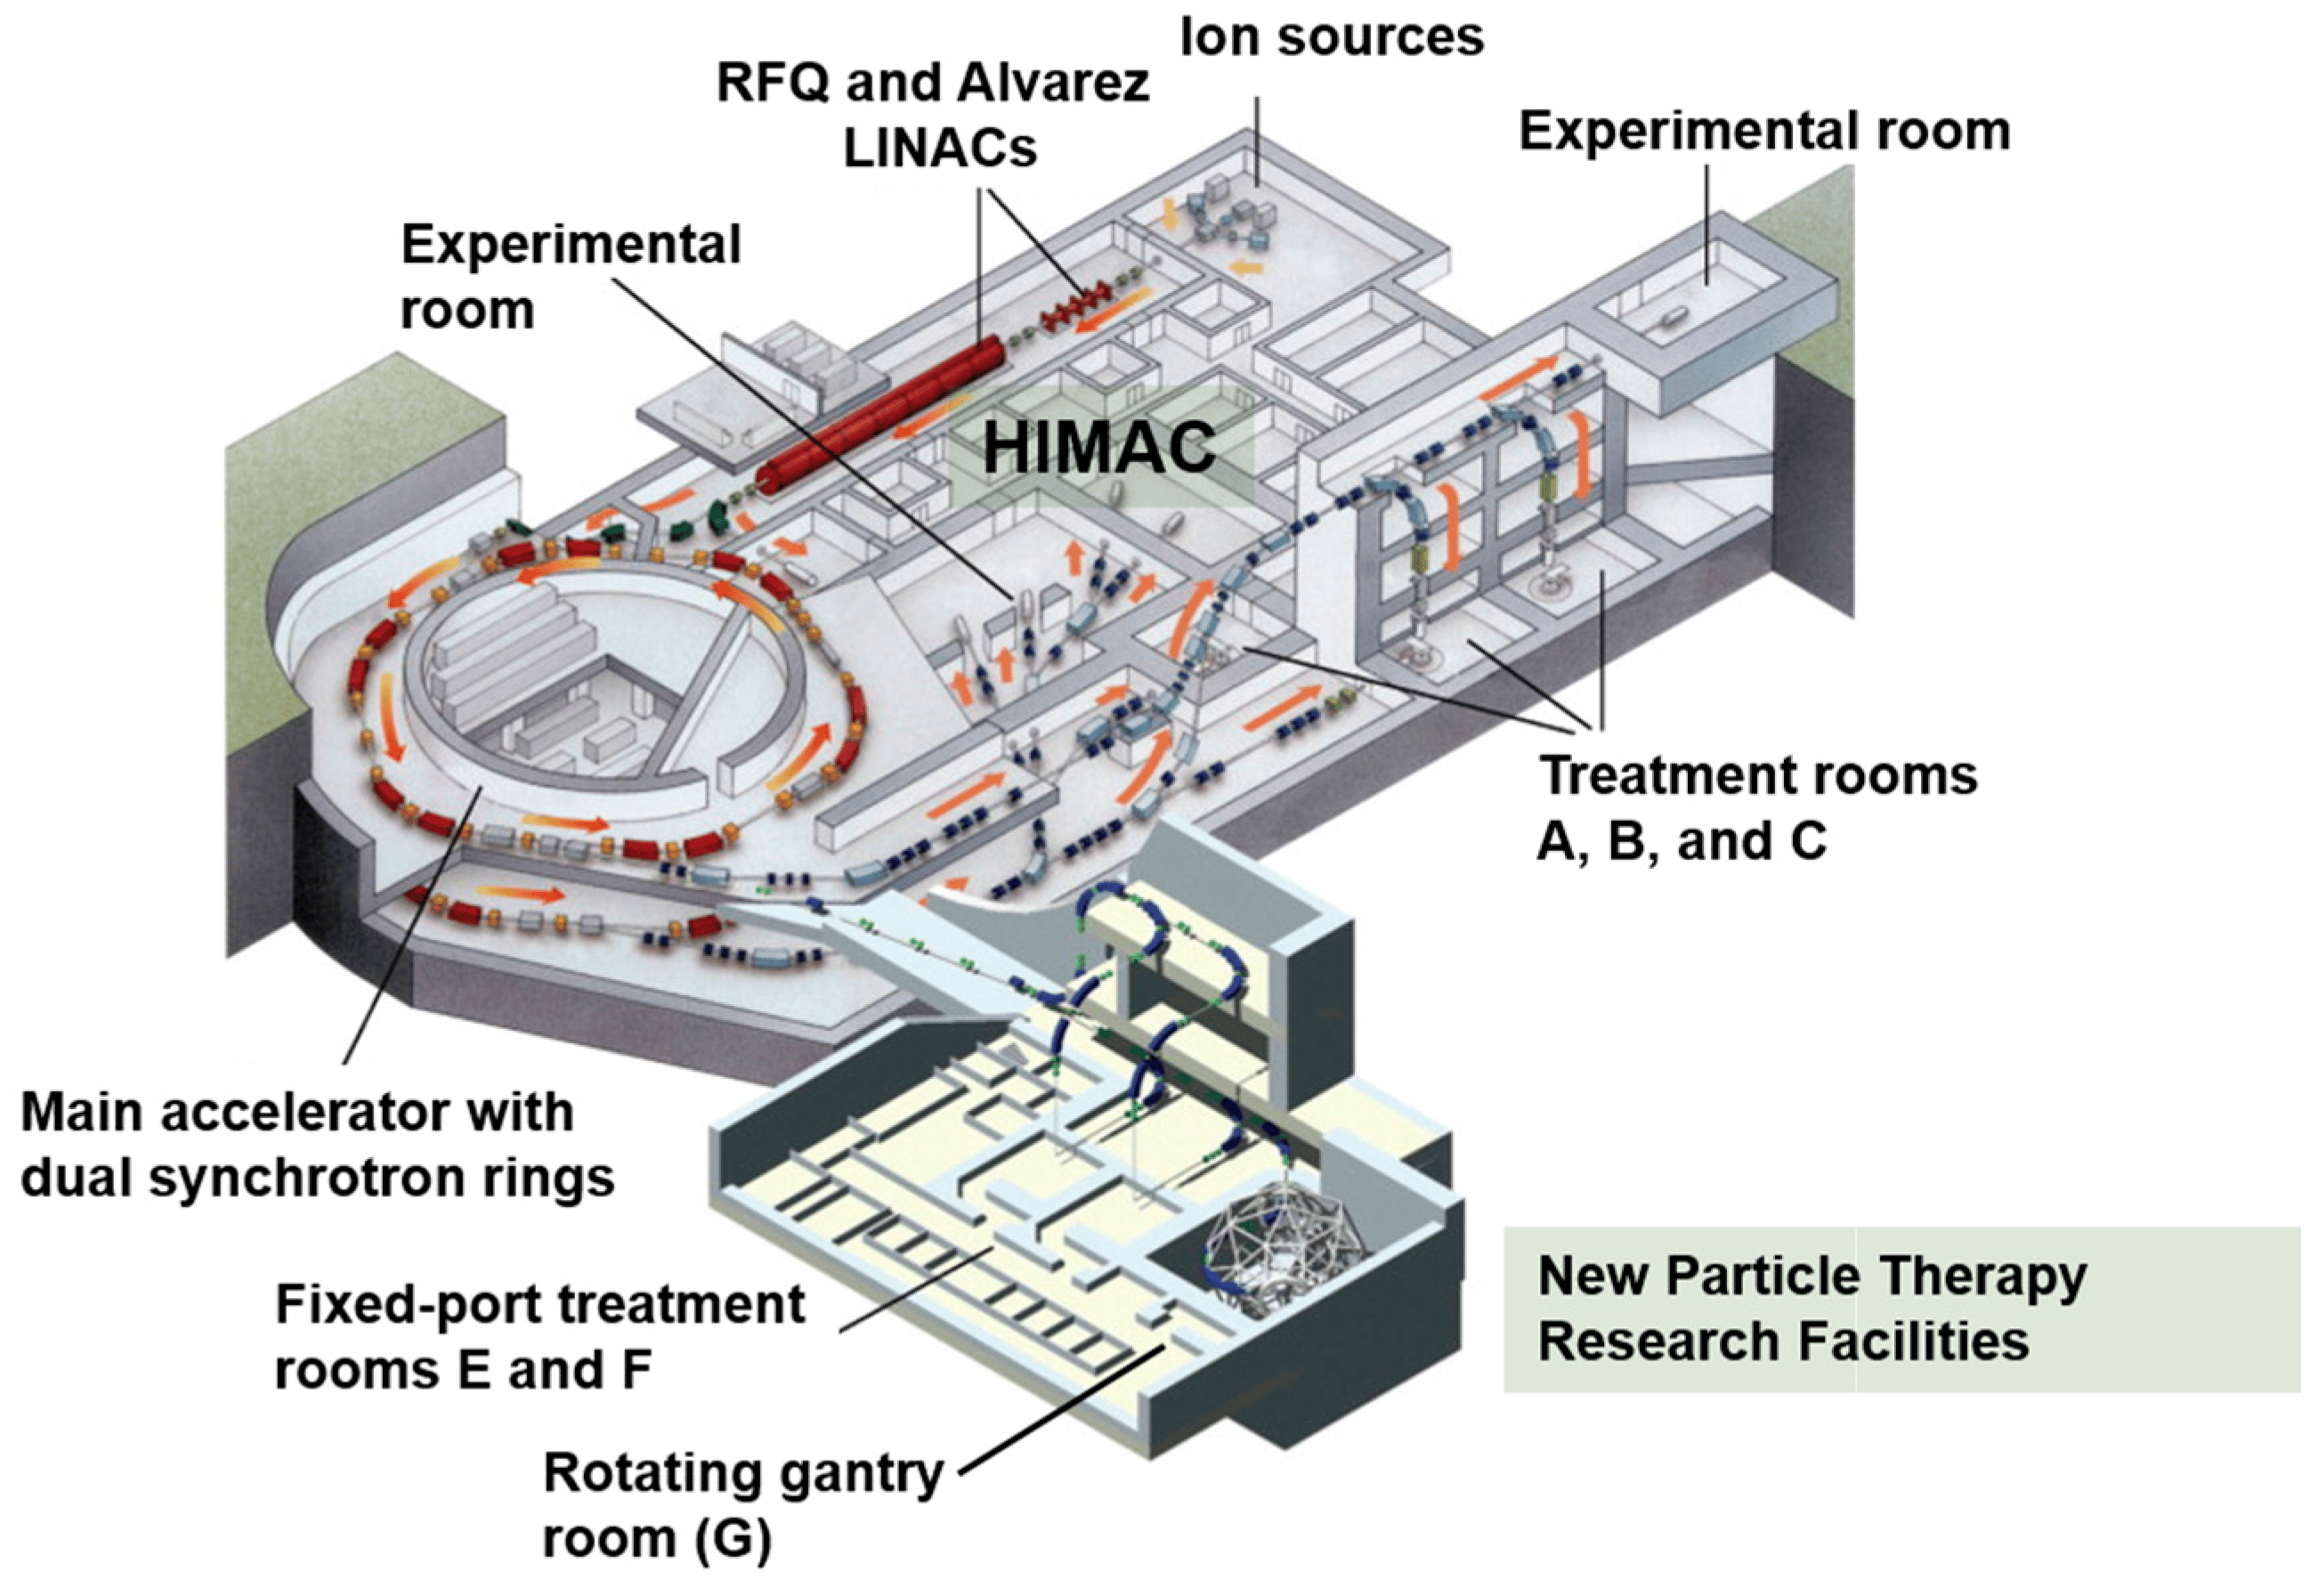
\includegraphics[width=0.9\linewidth]{images/himac.png}
		\caption{Panoramica delle strutture di ricerca HIMAC presso l'Istituto Nazionale di Scienze Radiologiche a Chiba (cita
			%https://www.mdpi.com/2072-6694/10/3/66
			).}
		\label{fig:himac}
	\end{figure}
	
	La prima iniziativa completamente europea di un centro terapico agli ioni arrivò solo nel $1987$ con EULIMA (EUropean Light Ion Medical Accelerator). Il progetto prevedeva la costruzione di un sincrotrone\footnote{I ciclotroni, con diametro di circa $5\mbox{ m}$, si utilizzano per produrre fasci di protoni, mentre i sincrotroni, con diametro di oltre $10\mbox{ m}$, si usano principalmente per generare ioni carbonio (cita
		%rivista asimmetrie, DOI 10.23801/asimmetrie.2023.35.03
	).} che, purtroppo, non fu mai costruito; si dovettero attendere progetti esclusivamente nazionali per un decisivo cambio di passo della terapia agli ioni, soprattutto nel decennio $1994$--$2004$, in cui iniziò la costruzione di due centri fondamentali per i trattamenti con protoni e ioni carbonio. Il primo è l'Heidelberg Ionenstrahl Therapy (HIT), aperto a Heidelberg (Germania) nel 2009, il secondo, italiano, è il Centro Nazionale di Adroterapia Oncologica (CNAO) di Pavia, attivo sin dal 2011 (cita
	%https://indico.cern.ch/event/24728/attachments/424989/590019/RIVISTA_MEDICA_2008-14_1.pdf ripetizione
	).
	
	\subsection{Adroterapia in Italia}
	Una delle figure più importanti per lo sviluppo dell'adroterapia in Italia è sicuramente il fisico italiano Ugo Amaldi ($1934$--). La sua lungimiranza ha portato l'Italia a essere la seconda nazione europea ad avere un centro adroterapico (il CNAO) capace di effettuare trattamenti con protoni e ioni carbonio (si pensi che attualmente ne esistono solo sei in tutto il mondo (cita
	%rivista asimmetrie, DOI 10.23801/asimmetrie.2023.35.03
	)). Nei paragrafi successivi si ripercorrono le principali tappe della storia dell'adroterapia in Italia.
	
	Nel $1991$, assieme al fisico medico Giampiero Tosi ($1937$--), Amaldi scrisse un articolo pionieristico in cui si proponeva un centro nazionale di terapia con particelle (cita
	%Amaldi U., Tosi G.: Per un centro di teleterapia con adroni. TERA 91/2, gen 2.
	), idea accolta con entusiasmo dal noto oncologo Umberto Veronesi ($1925$--$2016$) e dall'allora Presidente dell'Istituto Nazionale di Fisica Nucleare (INFN) Nicola Cabibbo ($1935$--$2010$). Un anno dopo, fu istituita la fondazione TERA (TErapia con Radiazioni Adroniche) con il duplice scopo di dare impiego a fisici e ingegneri interessati al progetto e di costruire centri adroterapici in Italia ed Europa (cita
	%https://indico.cern.ch/event/24728/attachments/424989/590019/RIVISTA_MEDICA_2008-14_1.pdf ripetizione
	).
	
	Alla fine del $1995$ si decise finalmente di creare una struttura protonterapica ai Laboratori Nazionali del Sud (LNS), sfruttando il ciclotrone superconduttore già attivo nei LNS. Il progetto, chiamato CATANA (Centro di AdroTerapia ed Applicazioni Avanzate, \hyperref[fig:catana]{Fig. 1.4}), prevedeva la collaborazione di INFN-LNS, Dipartimento di Fisica, Istituto di Oftalmologia e Radiologia dell'Università di Catania e il Centro Siciliano di Fisica Nucleare. Il ciclotrone catanese (\hyperref[fig:catana1]{Fig. 1.4a}), dotato di un complesso sistema dosimetrico in grado di misurare la dose entro un errore del $3\%$, accelerava fasci protonici a un'energia massima di $62 \mbox{ MeV}$, range adatto soprattutto per i tumori oculari (\hyperref[fig:catana2]{Fig. 1.4b}). Nel $2002$ si trattò il primo paziente affetto da melanoma uveale e da allora oltre $500$ pazienti hanno ricevuto trattamenti con successo per tumori intraoculari, melanomi congiuntivali e linfomi non Hodgkin.\footnote{I dati del $2014$, su un numero totale di $293$ pazienti, attestano un tasso di sopravvivenza del $98\%$ (cita
	%https://agenda.infn.it/event/8475/contributions/73755/attachments/53706/63315/1.Frascaticuttone.pdf
	), percentuale pur sempre comparabile con la terapia chirurgica e fotonica, sebbene queste ultime compromettano maggiormente la capacità visiva essendo statisticamente più invalidanti dell'adroterapia.}
	
	\begin{figure}[H]
		\centering
		\savebox{\largestimage}{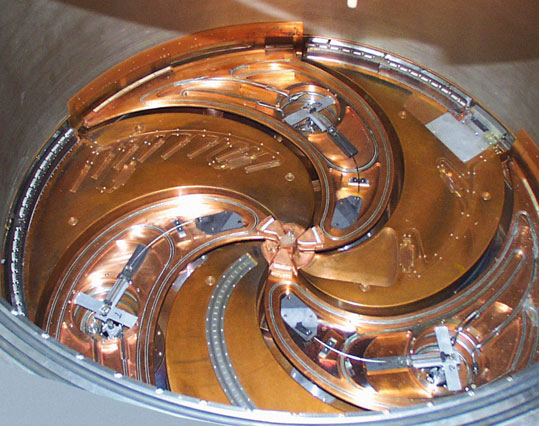
\includegraphics[width=0.49\textwidth]{images/catana1.jpg}}
		\begin{subfigure}[b]{0.49\textwidth}
			\centering
			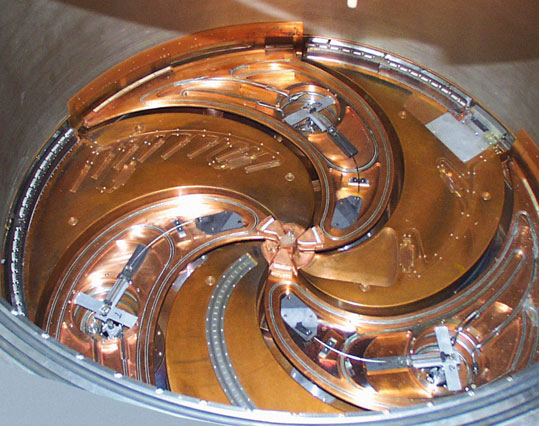
\includegraphics[width=\textwidth, scale=0.5]{images/catana1.jpg}
			\caption{Particolare interno del ciclotrone del CATANA (cita
				%rivista asimmetrie n.6 gli acceleratori
				).}
			\label{fig:catana1}
		\end{subfigure}
		\hfill
		\begin{subfigure}[b]{0.49\textwidth}
			\centering
			\raisebox{\dimexpr.5\ht\largestimage-.5\height}{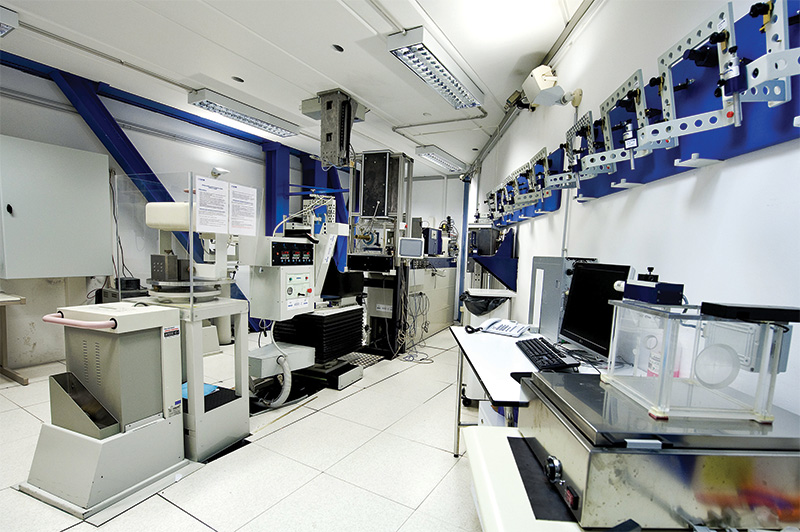
\includegraphics[width=\textwidth, scale=0.45]{images/catana2.jpg}}
			\caption{Attrezzatura presso la sala di trattamento del CATANA (cita
				%rivista asimmetrie, DOI: 10.23801/asimmetrie.2023.35.01
				).}
			\label{fig:catana2}
		\end{subfigure}
		\caption{Immagini relative al CATANA dei LNS, primo centro di protonterpia in Italia.}
		\label{fig:catana}
	\end{figure}
	
	Nel $1995$ Ugo Amaldi, con l'aiuto di Mainard Regler del progetto adroterapico austriaco Med-Austron, propose al direttivo del CERN (Conseil Européen pour la Recherche Nucléaire) di dare vita a PIMMS (Proton Ion Medical Machine Study) per la progettazione di un sincrotrone ottimizzato per il trattamento di tumori profondi attraverso ioni carbonio, protoni e altri ioni leggeri. PIMMS durò solo dal $1996$ al $2000$ ma fu un progetto talmente paradigmatico che, dopo ottimizzazioni successive, fornì una versione più compatta in termini di spazi e costi denominata PIMMS/TERA evolutasi nella versione CNAO definitivamente realizzata a Pavia (cita
	%https://fondazionecnao.it/storia
	). Proprio nel $2000$ il neoministro della Salute Umberto Veronesi autorizzò il finanziamento per la realizzazione del Centro Nazionale di Adroterapia (CNAO) e, nel maggio $2001$, istituì la Fondazione CNAO (cita
	%https://www.fondazioneveronesi.it/magazine/articoli/oncologia/potenzialita-e-limiti-delladroterapia
	). Dopo una prima fase di costruzione che ha coinvolto ben $500$ aziende italiane, Istituti ed Enti di Ricerca nazionali e internazionali, il CNAO si è attivato ufficialmente nel $2011$ (\hyperref[fig:edificio_cnao]{Fig. 1.5a}). La terapia adroterapica del CNAO, come già accennato, avviene accelerando protoni e ioni carbonio rispettivamente fino a un'energia cinetica di $250 \mbox{ MeV}$ e $4800\mbox{ MeV}$ (circa $400\mbox{ MeV/u}$\footnote{$\mbox{ MeV/u}$ è l'unità di misura dell'energia per unità di massa atomica.}). I trattamenti si svolgono in tre sale, due delle quali richiedono un fascio orizzontale mentre la terza consente un irraggiamento sia orizzontale che verticale (\hyperref[fig:sala_cnao]{Fig. 1.5b}). Protoni e ioni carbonio vengono accelerati a circa $30000\mbox{km/s}$ da un sincrotrone a forma di anello avente $25\mbox{ m}$ di diametro e $80\mbox{ m}$ di circonferenza (\hyperref[fig:sincrotrone_cnao]{Fig. 1.5c}). Gli attuali obiettivi del CNAO non sono solo quelli di arrivare a trattare circa $700$ pazienti all’anno, ma anche di diventare l’unico centro di adroterapia al mondo a disporre di protoni, ioni carbonio, altre specie ioniche e BNCT (Boron Neutron Capture Therapy) ?aggiungere riferimento alla BNCT? (cita
	https://fondazionecnao.it/futuro-scopri-progetto-espansione-cnao/gianluca-vago
	).
	
	\begin{figure}[H]
		\centering
		\subfloat[Edificio sanitario del complesso edilizio del CNAO contenente servizi sanitari, amministrativi e di alta tecnologia come il sincrotrone (cita
		%https://www.bimportale.com/cnao-centro-nazionale-adroterapia-oncologica/
		).]{\label{fig:edificio_cnao}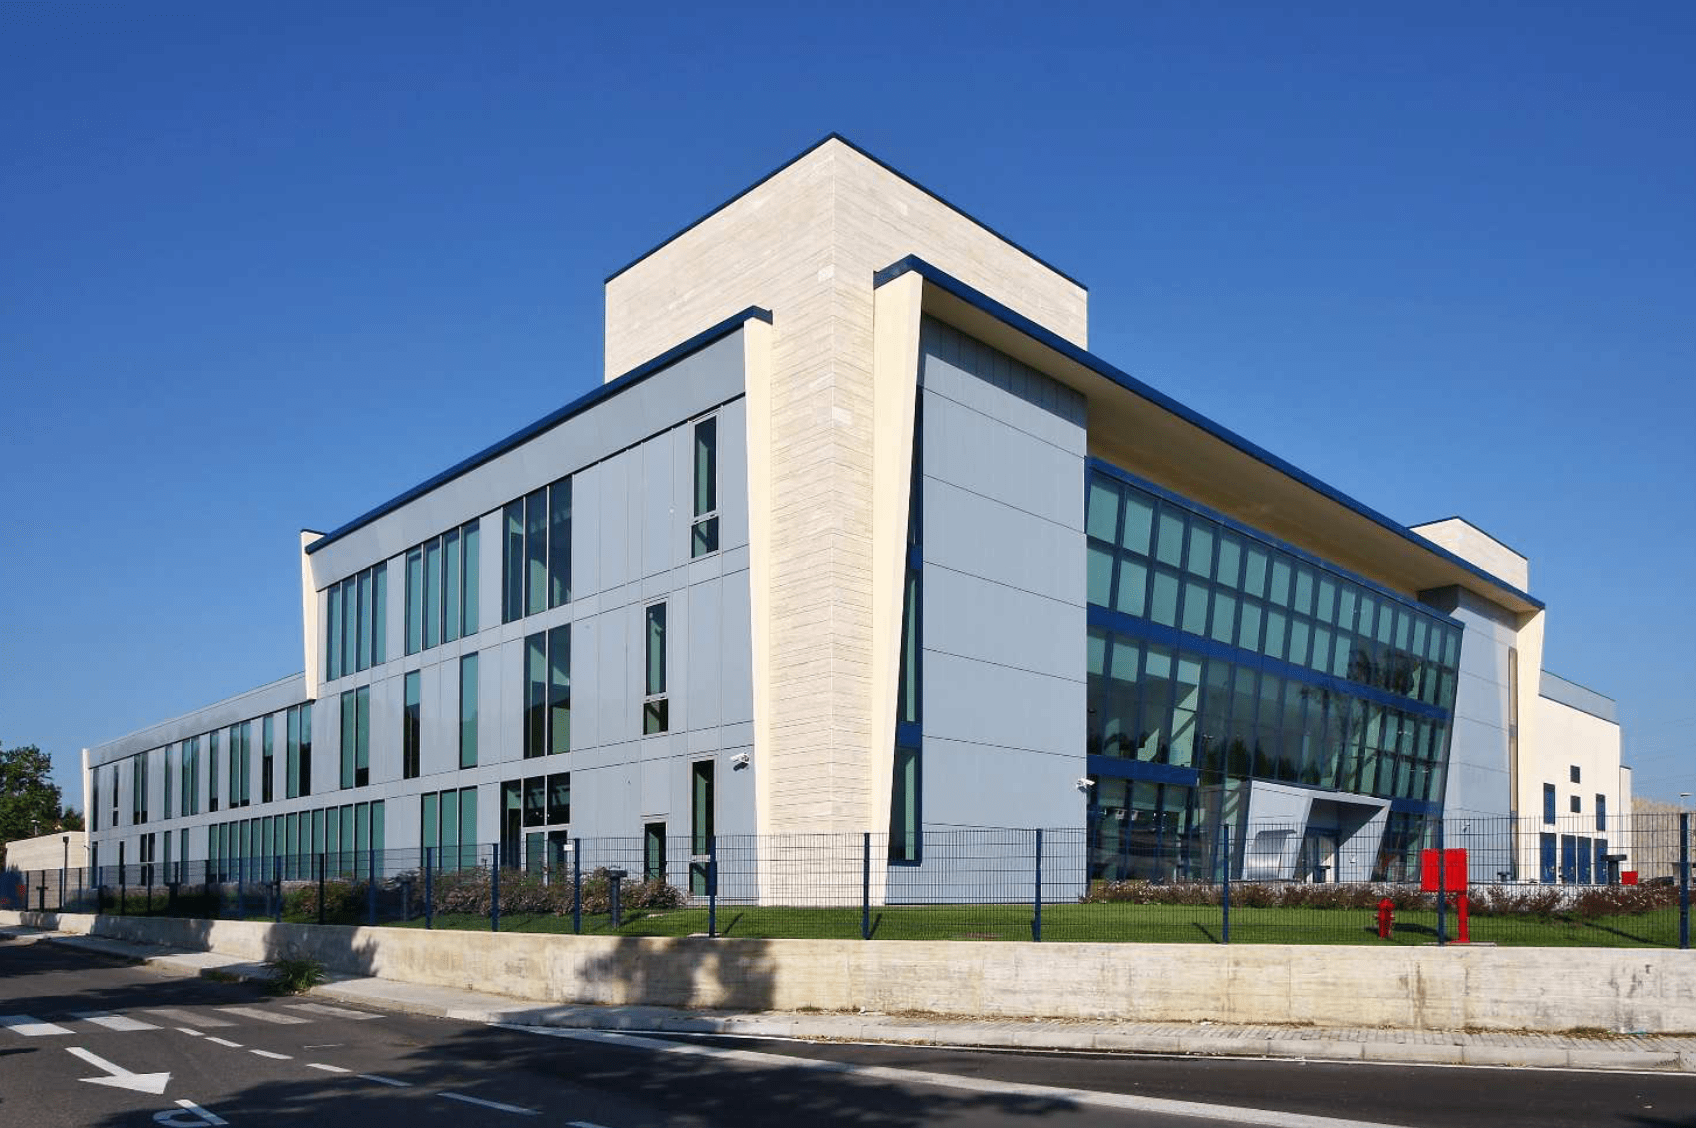
\includegraphics[width=.49\linewidth]{images/edificio_cnao.jpg}}\hfill
		\subfloat[Una delle sale di trattamento del CNAO. Il fascio è in grado di raggiungere il paziente sia dall'alto che da sinistra (cita
		%rivista asimmetrie, DOI 10.23801/asimmetrie.2023.35.03
		).]{\label{fig:sala_cnao}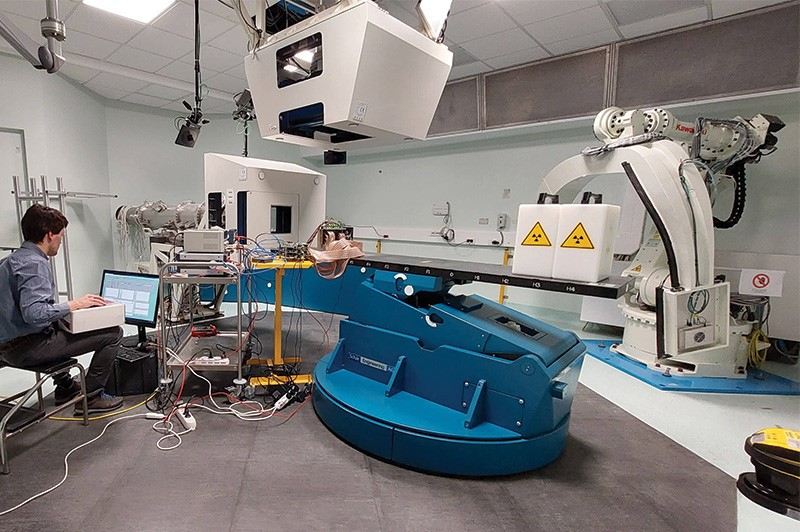
\includegraphics[width=.49\linewidth]{images/sala_cnao.jpg}}\par 
		\subfloat[Il sincrotrone del CNAO, situato in un bunker di $1600\mbox{ m}^2$ isolato dal resto della struttura con spesse pareti in cermento armato (cita
		%https://www.facebook.com/photo/?fbid=2533501746969553&set=a.1378679705785102
		).]{\label{fig:sincrotrone_cnao}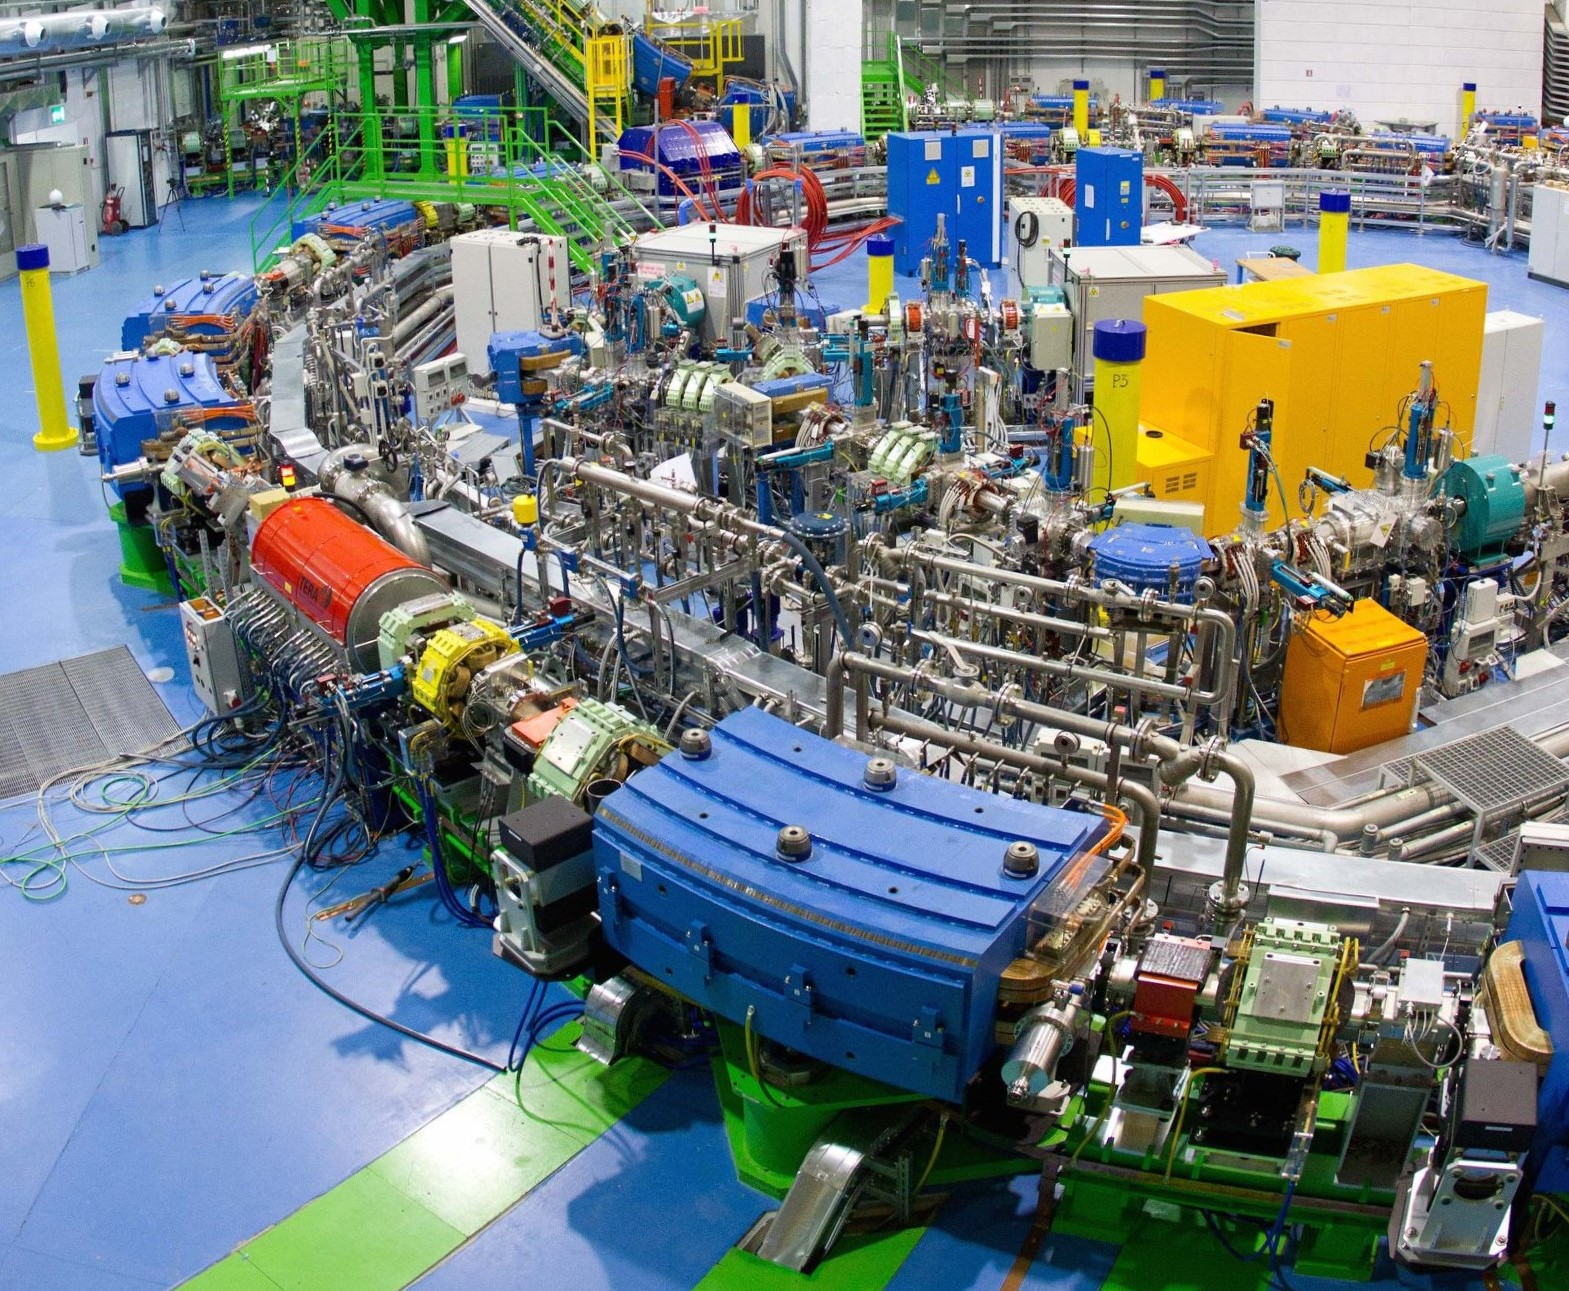
\includegraphics[width=.49\linewidth]{images/sincrotrone_cnao.jpg}}
		\caption{Immagini relative al CNAO di Pavia.}
		\label{fig:cnao}
	\end{figure}
	
	Il centro adroterapico italiano più recente è il Proton Therapy Center (PTC) di Trento, la cui attività clinica ha avuto inizio nell'ottobre del 2014 (cita
	%https://protonterapia.provincia.tn.it/eng
	). Il PCT, che è una delle unità operative del Dipartimento di Oncologia dell'Ospedale di Trento, utilizza solo fasci di protoni accelerati da un ciclotrone a un'energia di $70$--$226 \mbox{ MeV}$ (cita
	%trentoPCT.pdf
	). Uno dei punti di forza del PCT è la sua capacità di erogare protoni per mezzo di sistemi rotanti (gantry, \hyperref[fig:gantry]{Fig. 1.6}), garantendo un trattamento del paziente full-body a $360^\circ$ per patologie come tumori cerebrali e della base cranica, del distretto cervico-cefalico, della colonna vertebrale, sarcomi dei tessuti molli e tumori pediatrici (cita
	%https://www.apss.tn.it/Azienda/Unita-operative-e-strutture-organizzative/Unita-operativa-protonterapia-Trento#cosa_fa
	). Inoltre il centro adroterapico trentino è il primo in Italia a erogare un fascio di protoni in modalità attiva; quest'ultima, a differenza delle modalità uniforme e passiva, utilizza campi magnetici per deviare il percorso di ciascun fascio di protoni verso la posizione target, determinata subito prima che la dose venga erogata (cita	%https://www.radioterapiaitalia.it/wp-content/uploads/2017/03/Amichetti-Proton-parte-1.pdf
	,
	%https://www.ncbi.nlm.nih.gov/pmc/articles/PMC4651068/
	).
	
	\begin{figure}[H]
		\centering
		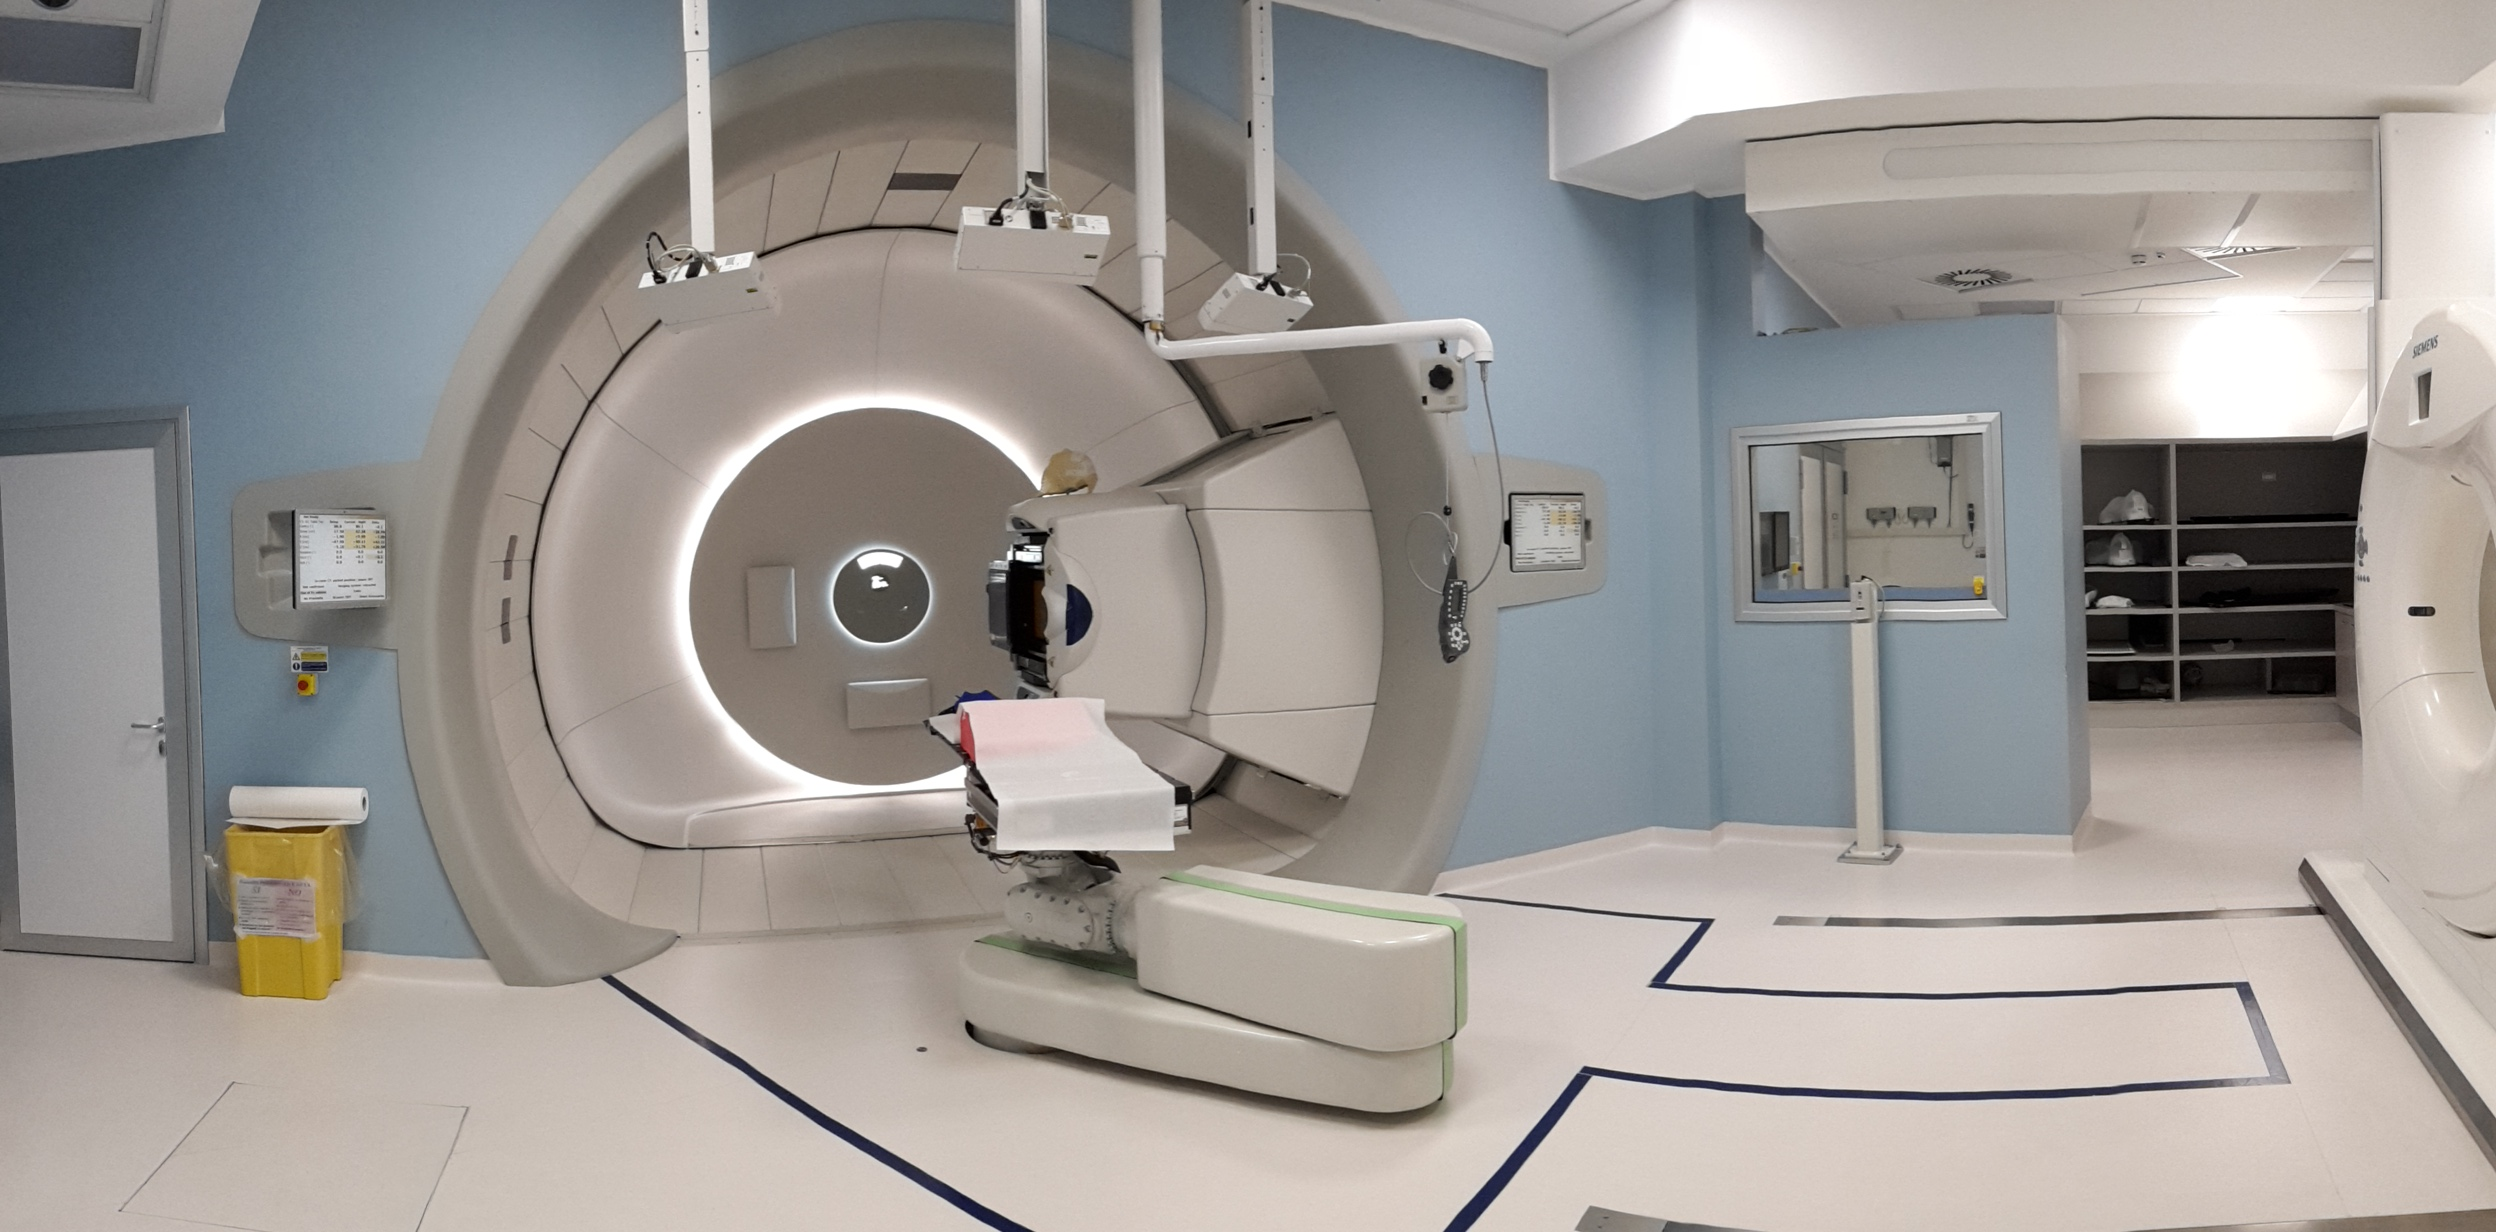
\includegraphics[width=0.9\linewidth]{images/gantry.jpg}
		\caption{Gantry Blu del Centro di Protonterapia di Trento (cita
			%https://it.wikipedia.org/wiki/Protonterapia
			).}
		\label{fig:gantry}
	\end{figure}
	
	Il PCT possiede due linee protoniche dedicate ai trattamenti clinici dotate di gantry e una linea fissa utilizzata per attività sperimentali di ricerca e sviluppo (R\&D). Le attività di R\&D non sono legate esclusivamente alla protonterapia ma anche a contesti lontani dall'ambito medico, per esempio gli ambiti aerospaziale con la radioprotezione (si veda \hyperref[label]{radioprotezione}) ed elettronico con lo studio di componenti elettroniche radioresistenti, l'analisi dei materiali e lo sviluppo di rivelatori (cita
	%https://protonterapia.provincia.tn.it/Per-i-ricercatori?/eng/switchlanguage/to/protonterapia_frontend/researchers
	). 
	
	\subsubsection{Tecniche e R\&S nel percorso radioterapico}
	Prima di ogni trattamento, i moderni centri radio e adroterapici compiono un attento percorso di pianificazione del trattamento (TP, Treatment Planning), l'anello iniziale di ogni percorso radioterapico. La TP  include numerosi passaggi fondamentali tra cui la topologia del volume tumorale tramite tecniche di imaging diagnostico morfologico e funzionale come TAC (Tomografia Assiale Computerizzata), RMN (Risonanza Magnetica Nucleare), PET (Tomografia a Emissione di Positroni) e SPECT (Tomografia a Emissione di Singolo Fotone), strumenti che con lo sviluppo tecnologico hanno acquisito una sensibilità sempre maggiore fornendo mappe tridimensionali dei tessuti del corpo umano ancora più dettagliate. Compito del TP è anche quello di pianificare la dose totale a cui sottoporre il paziente, congiuntamente al suo rateo e al suo frazionamento; ad esempio, al CNAO per i protoni in media sono necessarie 35 sedute mentre per gli ioni carbonio 16 (cita
	%https://fondazionecnao.it/adroterapia/sincrotrone
	).
	
	Attualmente, gli obiettivi principali dell'adroterapia sono quelli di migliorare il dosaggio della radiazione nel paziente, tenendo conto anche del suo movimento respiratorio durante la seduta, e di comprendere gli effetti delle radiazioni sul corpo umano. Per questo motivo, è fondamentale implementare l'efficacia dei rivelatori in grado di misurare l'irraggiamento dei fasci adronici, sviluppare micro e nano-dosimetri per consentire un minuzioso rilascio della dose, teorizzare modelli matematici che leghino la sopravvivenza cellulare con il tipo di irraggiamento radioterapico ricevuto, studiare tecniche di imaging ricostruttivo in grado di misurare i cambiamenti anatomici che il tumore e gli organi limitrofi possono subire anche in breve tempo. Gli sviluppi sopra elencati richiedono il lavoro congiunto di oncologi, radiologi e fisici che uniscono imprescindibili competenze in radiobiologia, elettronica, fisica dei materiali e computing. In particolare, al giorno d'oggi si sfruttano copiosamente sistemi di calcolo avanzati, metodi di intelligenza artificiale (come algoritmi di deep learning e machine learning) e simulazioni Montecarlo in grado di compiere analisi predittive e adattive, divenute ormai fondamentali nel contesto applicativo delle scienze omiche (cita
	%rivista asimmetrie, DOI 10.23801/asimmetrie.2023.35.01
	,
	%rivista asimmetrie, DOI 10.23801/asimmetrie.2023.35.02
	,
	%rivista asimmetrie, DOI 10.23801/asimmetrie.2023.35.03
	).
	
	\section{Parametri fisici ed effetti biologici della radiazione}
	Come descritto nella \hyperref[sec:1.1]{Sez. 1.1}, le cellule tumorali generano un disequilibrio dell'omeostasi dell'organismo umano poiché, a differenza delle cellule sane, sfuggono a meccanismi di controllo che limitano la loro proliferazione, una regolazione che avviene automaticamente nelle in condizioni normali. Infatti, molte cellule malate possiedono sistemi di controllo difettosi che non permettono di arrestare il ciclo cellulare nei punti di controllo\footnote{I punti di controllo sono stadi del ciclo cellulare in cui quest'ultimo subisce automaticamente un arresto, in attesa che arrivi un segnale che permetta la sua prosecuzione.} nemmeno quando sono assenti i fattori di crescita\footnote{I fattori di crescita sono proteine che stimolano la divisione di alcune cellule} (cita
	% libro biologia III anno
	).
	
	Le alterazioni del ciclo cellulare sono generalmente causate da disfunzioni dell'espressione genica (\hyperref[fig:mutazioni_genetiche]{Fig. 1.7}), che è il processo con cui l'informazione contenuta nei geni fluisce alle proteine (le macromolecole funzionali del nostro corpo) per mezzo di meccanismi di trascrizione e traduzione del DNA.\footnote{Ogni gene è costituito da centinaia o migliaia di nucleotidi.} I geni modificati capaci di generare cellule tumorali sono denominati oncogeni. Generalmente le cellule sane acquisiscono un oncogene a partire da una mutazione di uno dei propri geni, chiamato proto-oncogene. Il cromosoma degli esseri umani contiene proto-oncogeni, la cui funzione in condizioni ordinarie è quella di codificare per fattori di crescita o per altre funzioni del ciclo cellulare, che potenzialmente possono tramutarsi in oncogeni tramite mutazioni, errori di duplicazione o ricombinazione del DNA e traslocazioni in \textit{loci} genici soggetti a fattori di controllo che ne inducono la trascrizione a ritmi più elevati del normale (\hyperref[fig:oncogene]{Fig. 1.7a}). Oltre ai proto-oncogeni, che stimolano la divisione cellulare, esistono gli oncosoppressori, geni che codificano per proteine che inibiscono la proliferazione cellulare incontrollata. Per questo motivo le mutazioni che riducono le attività delle proteine codificate dai geni oncosoppressori possono portare all'insorgenza di un tumore (\hyperref[fig:oncosoppressore]{Fig. 1.7b}). Il fatto che le neoplasie siano originate da danni genetici è un'ipotesi ampiamente accettata che si basa su considerazioni come il riconoscimento di una predisposizione ereditaria al cancro, il ritrovamento di cromosomi danneggiati in cellule cancerose e il rapporto fra suscettibilità al cancro e incapacità delle cellule a riparare il DNA danneggiato (cita
	%https://www.treccani.it/enciclopedia/oncogeni_(Enciclopedia-Italiana)/
	). Per esempio, si pensi che le mutazioni di due noti geni \textit{ras} (proto-oncogene) e \textit{p53} (gene oncosoppressore) sono rilevate rispettivamente nel $30\%$ e in più del $50\%$ dei casi di cancro umano (cita
	% libro biologia III anno
	).
	
	\begin{figure}[H]
		\centering
		\begin{subfigure}[b]{0.9\textwidth}
			\centering
			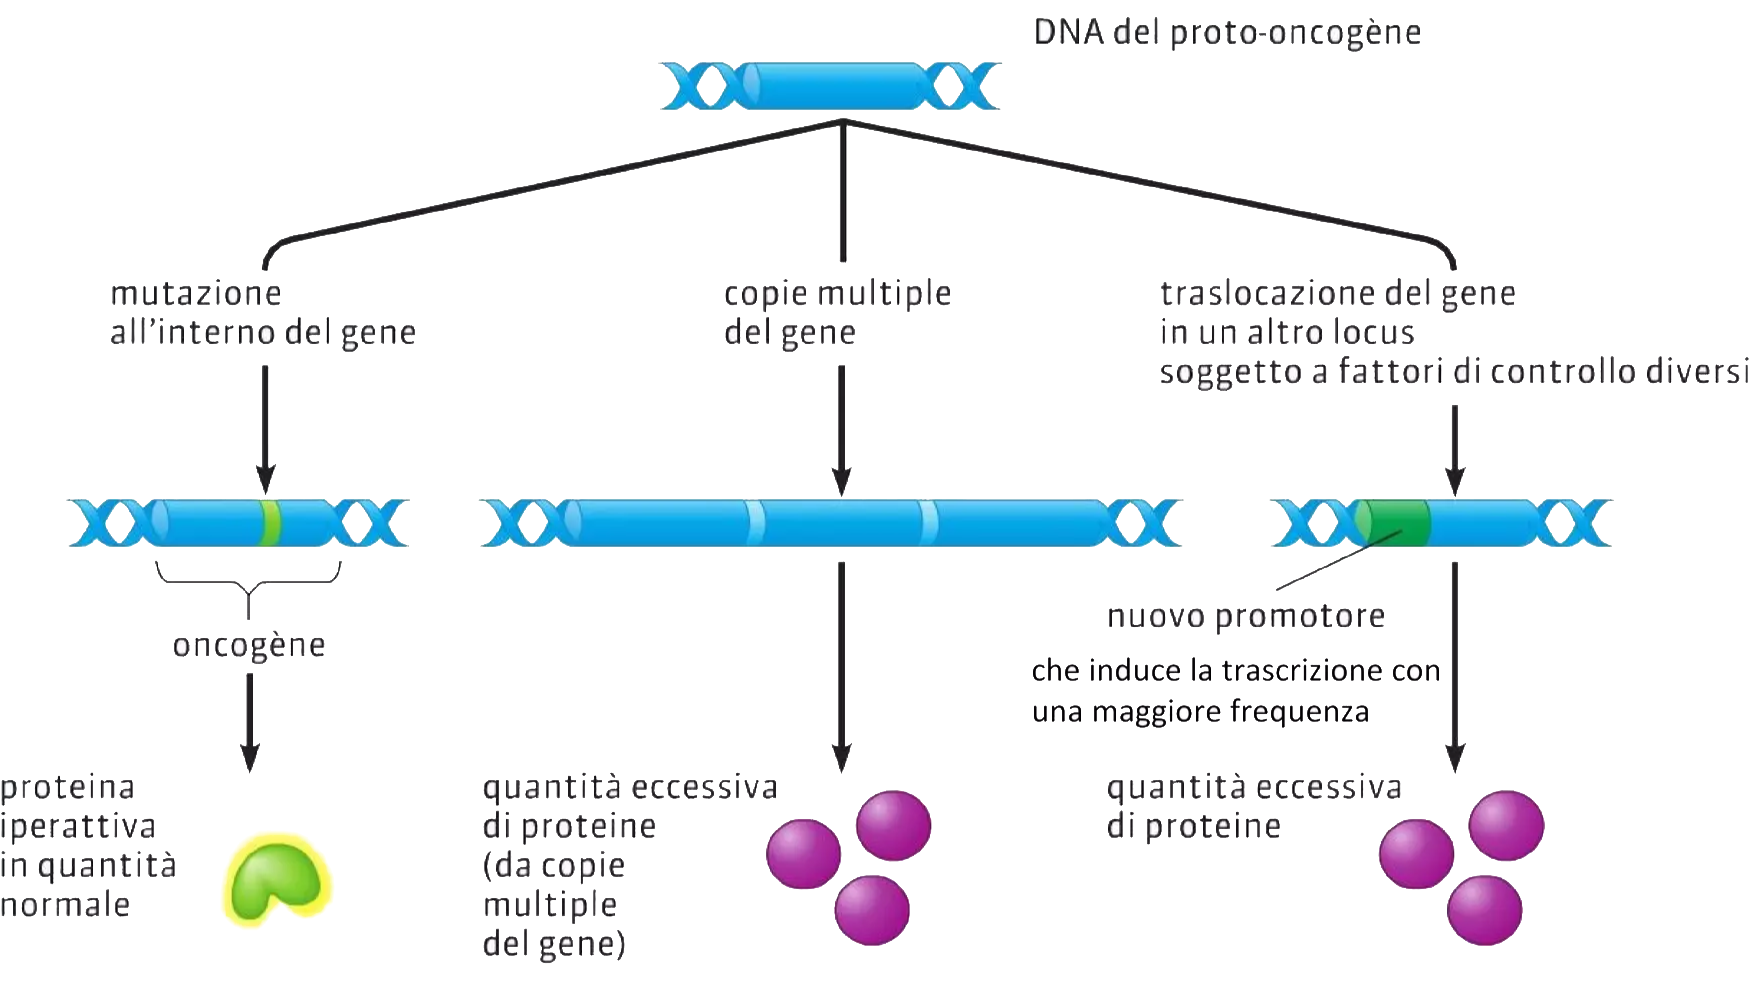
\includegraphics[width=\textwidth, scale=0.5]{images/oncogene.png}
			\caption{Modalità con cui un proto-oncogene può mutare in un oncogene.}
			\label{fig:oncogene}
		\end{subfigure}
		\par
		\begin{subfigure}[b]{0.9\textwidth}
			\centering
			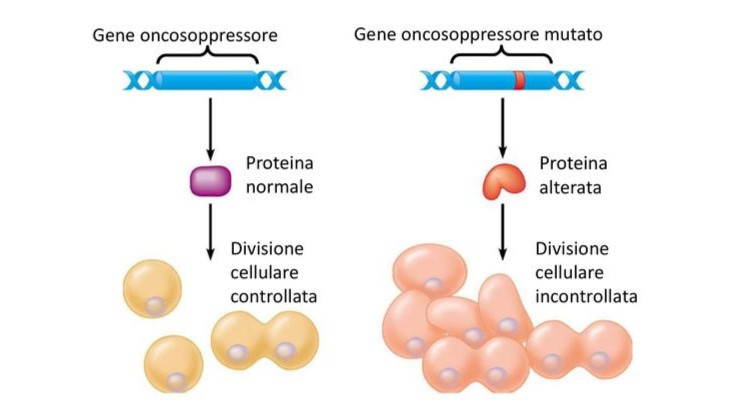
\includegraphics[width=\textwidth, scale=0.45]{images/oncosoppressore.jpg}
			\caption{Effetto della mutazione di un gene oncosoppressore.}
			\label{fig:oncosoppressore}
		\end{subfigure}
		\caption{Esempi di mutazioni subite da geni che controllano la divisione cellulare (cita
			%II anno libro biologia
			).}
		\label{fig:mutazioni_genetiche}
	\end{figure}
	
	\subsection{Danni biologici delle radiazioni ionizzanti}
	La radioterapia e l'adroterapia, come descritto in \hyperref[sec:1.2]{Sez. 1.2}, sfruttano la radiazione ionizzante per danneggiare i tessuti biologici cancerosi al fine di causare la morte delle cellule malate che li costituiscono. La ionizzazione può essere generata direttamente o indirettamente: se vi è un'interazione diretta tra la radiazione incidente e gli elettroni dell'atomo irradiato allora si parla di radiazione direttamente ionizzante, altrimenti se vi è un'interazione tra gli atomi irradiati e particelle secondarie (generate dal passaggio della radiazione primaria) allora si ha radiazione indirettamente ionizzante. Tra le radiazioni direttamente ionizzanti si riconoscono le particelle $\alpha$ e $\beta$, mentre del secondo caso fanno parte raggi $\gamma$ X e particelle neutre come i neutroni. La radiazione ionizzante produce vari effetti sui tessuti biologici (si veda \hyperref[qualcosa]{???}) che dipendono da svariati fattori, tra cui l'energia del fascio incidente, la sua composizione e le caratteristiche del tessuto irradiato. Per comprendere i danni biologici che la radiazione provoca sui tessuti cancerosi è opportuno analizzare ciò che accade a livello cellulare.
	
	Per le cellule tumorali si parla di morte riproduttiva nel momento in cui la cellula perde la sua capacità di riprodursi indefinitamente (cita
	%https://www.unife.it/medicina/radiologiamedica/insegnamenti/scienze-biologiche-nella-radiologia/modulo-di-radiobiologia/cittanti-2018-19-colori/rb-2018-19-lezione-6
	). Per sconfiggere una neoplasia non occorre eliminare tutte le cellule tumorali, piuttosto è necessario impedire alla cellula di riprodursi per mitosi (o meiosi se si tratta di una cellula deputata alla riproduzione (cita
	%libro biologia II anno
	)) mediante la distruzione del DNA contenuto nel suo nucleo. Per uccidere il DNA cellulare tramite radiazione ionizzante vi sono due modi, diretto e indiretto, descritti nei prossimi paragrafi.
	
	\subsubsection{Danno diretto}
	Prima di analizzare il danno diretto che la radiazione può arrecare al DNA, è opportuno descrivere la struttura e le funzioni di quest'ultimo. Il DNA (acido desossiribonucleico) è un polimero costituito da monomeri chiamati nucleotidi, molecole a loro volta composte da una base azotata, uno zucchero e un gruppo fosfato, esaminate in \hyperref[fig:nucleotide]{Fig. 1.8}. Esistono quattro tipi di nucleotidi, la cui specificità è data dal tipo di base azotata: adenina (A), citosina (C), timina (T) o guanina (G).
	
	\begin{figure}[H]
		\centering
		\includegraphics[width=0.9\linewidth]{images/nucleotide.pdf}
		\caption{Nucleotide formato a sinistra da un gruppo fosfato contenente un atomo di fosforo \ce{P} (che determina il carattere acido degli acidi nucleici), al centro da uno zucchero (desossiribosio) formato da cinque atomi di carbonio e in alto a destra da una base azotata contenente un gruppo \ce{\bond{-}NH} (che conferisce loro un carattere basico) legata con lo zucchero per mezzo di un legame glicosidico.(a sinistra)o zucchero cinque (cita
			%https://en.wikipedia.org/wiki/Nucleotide
			).}
		\label{fig:nucleotide}
	\end{figure}
	
	Oltre al DNA esiste anche l'RNA (acido ribonucleico), un acido nucleico fondamentale per la biosintesi delle proteine. Nonostante DNA e RNA siano entrambi costituiti da una lunga catena nucleotidica, presentano varie differenze strutturali e funzionali:
	
	\begin{itemize}
		\item il DNA ha una struttura di doppia elica (caratterizzata dal diametro costante di $2\mbox{ nm}$ (cita
		%libro 3 anno CAMPBELL
		)) costituita da due catene nucleotidiche antiparallele (legate tramite legami idrogeno che intercorrono tra A e T oppure tra C e G), mente l'RNA è formato da una singola elica in cui la timina (T) viene sostituita dall'uracile (U) (\hyperref[fig:dna_structure]{Fig. 1.9});
		\item lo zucchero del DNA (desossiribosio) possiede un atomo di ossigeno in meno rispetto al ribosio dell'RNA;
		\item nelle cellule eucariote, il DNA è collocato nel nucleo mentre l'RNA si trova sia nel nucleo che nel citoplasma;
		\item il DNA è depositario dell'informazione genetica mentre l'RNA è l'intermediario tra il DNA e la sintesi di proteine specifiche.
	\end{itemize}
	
	La scoperta delle strutture degli acidi nucleici DNA e RNA (\hyperref[fig:dna_structure]{Fig. 1.9}) viene attribuita agli scienziati James D. Watson ($1928$--), Francis H. C.Crick ($1916$--$2004$) e Maurice H. F. Wilkins ($1916$--$2004$) che per il loro contributo alla biologia molecolare ricevettero il premio Nobel per la fisiologia o la medicina nel $1958$. In realtà la prima immagine cristallografica del DNA fu quella della chimica Rosalind E. Franklin ($1920$--$1958$), anche se per molto tempo non gli fu riconosciuta la paternità della scoperta. Purtroppo la sua morte precoce non le consentì nemmeno di essere candidata al premio Nobel (cita
	%libro 3 anno CAMPBELL
	).
	
	\begin{figure}[H]
		\centering
		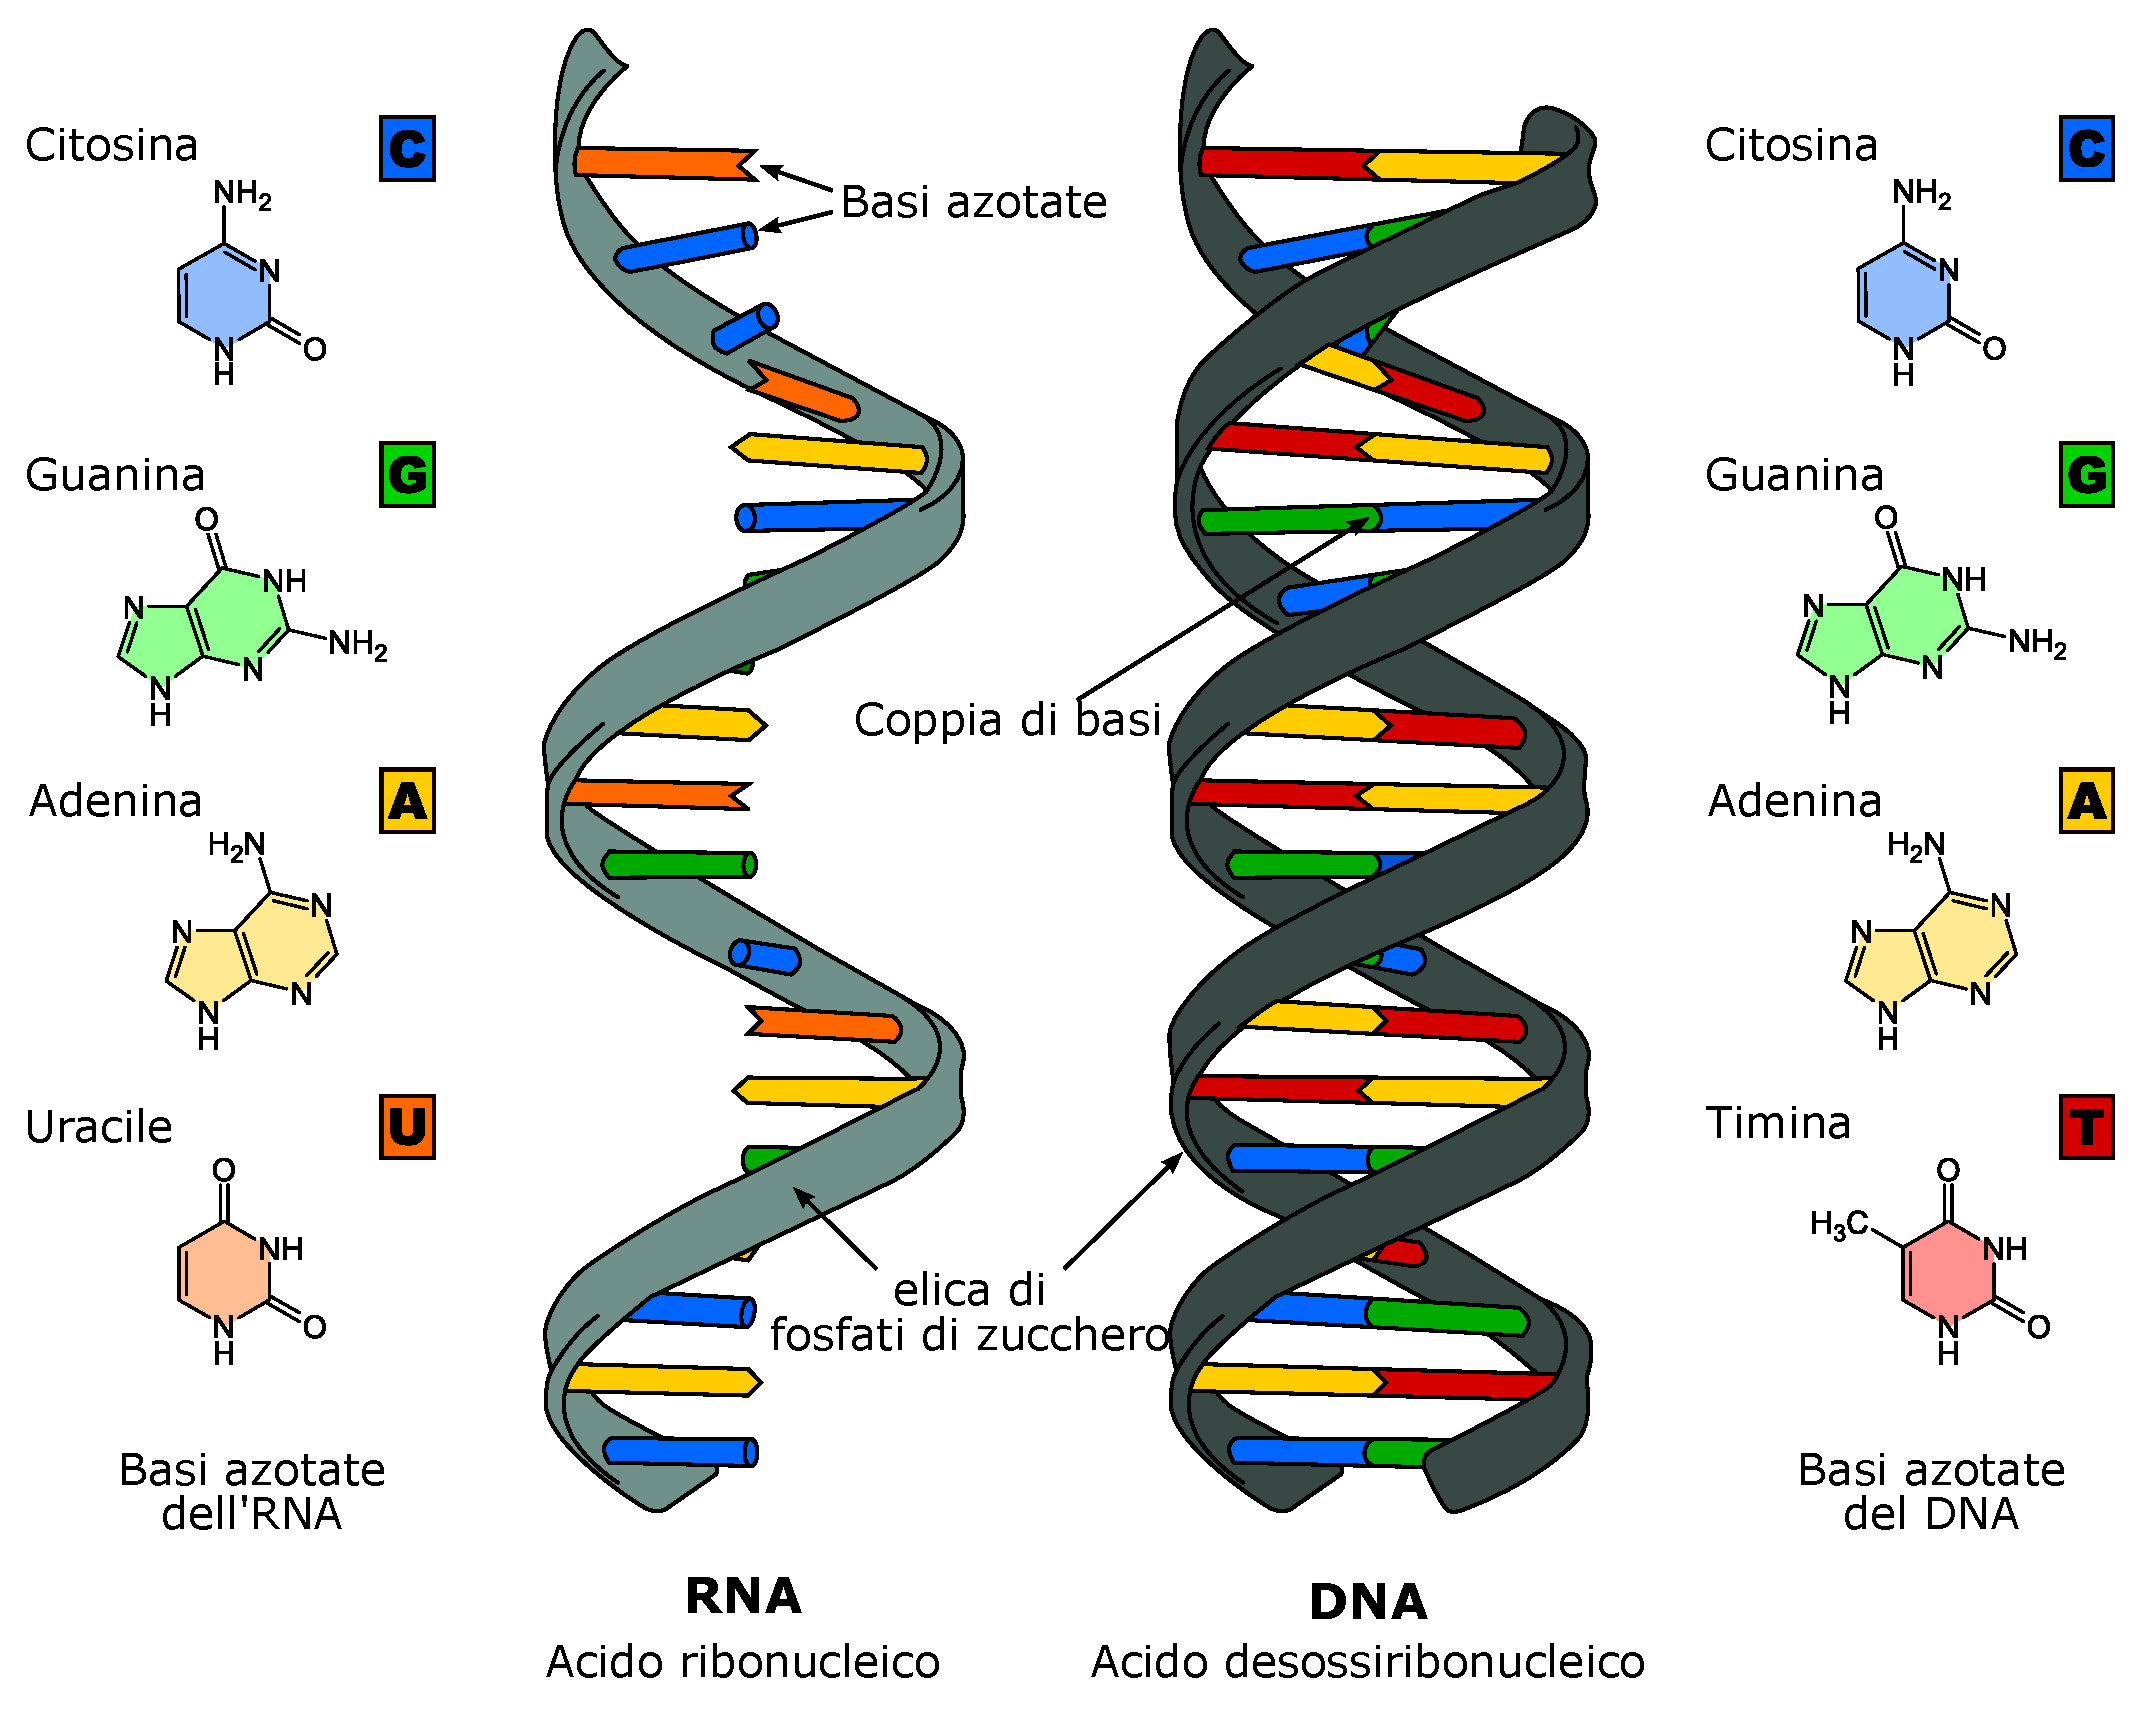
\includegraphics[width=0.9\linewidth]{images/dna_structure.pdf}
		\caption{Struttura a singola elica dell'RNA e a doppia elica del DNA con relativi accoppiamenti delle basi azotate (cita
		%https://it.wikipedia.org/wiki/Acidi_nucleici
		).}
		\label{fig:dna_structure}
	\end{figure}
	
	Come parzialmente accennato in precedenza, le funzioni del DNA sono quelle di regolare la riproduzione delle cellule (mediante la sua duplicazione che favorisce la trasmissione delle informazioni ereditarie) e di controllare l'espressione genica. In particolare, il dogma centrale della biologia molecolare (proposto nel $1956$ dallo stesso Francis Crick (cita
	%libro campbell3 anno
	)) prevede che le fasi principali della sintesi proteica siano la trascrizione e la traduzione (\hyperref[fig:dna_rna]{Fig. 1.10}). Durante la trascrizione si genera un filamento di mRNA (RNA messaggero) le cui basi azotate sono complementari a quelle della molecola di DNA che è utilizzata come stampo. Durante la traduzione avviene un "cambiamento di linguaggio" in cui l'informazione genica contenuta nel DNA (per mezzo dell'mRNA, dell'tRNA (RNA di trasporto) e dei ribosomi) viene tradotta da una sequenza di nucleotidi in una sequenza di amminoacidi, i "mattoni" che costituiscono le proteine. Nello specifico, ad ogni tripletta di basi azotate (denominata codone) corrisponde un amminoacido (la totalità delle $4^3=64$ combinazioni consente di codificare per tutti i 20 amminoacidi esistenti in natura). Eventuali variazioni della sequenza nucleotidica (come la sostituzione, l'inserzione o la delezione di una base azotata) generano le mutazioni che, in mancanza dei meccanismi di controllo cellulare, sono la causa di molti disturbi e malattie ereditarie (cita
	%libro 3 anno biologia campbell
	).
	
	\begin{figure}[H]
		\centering
		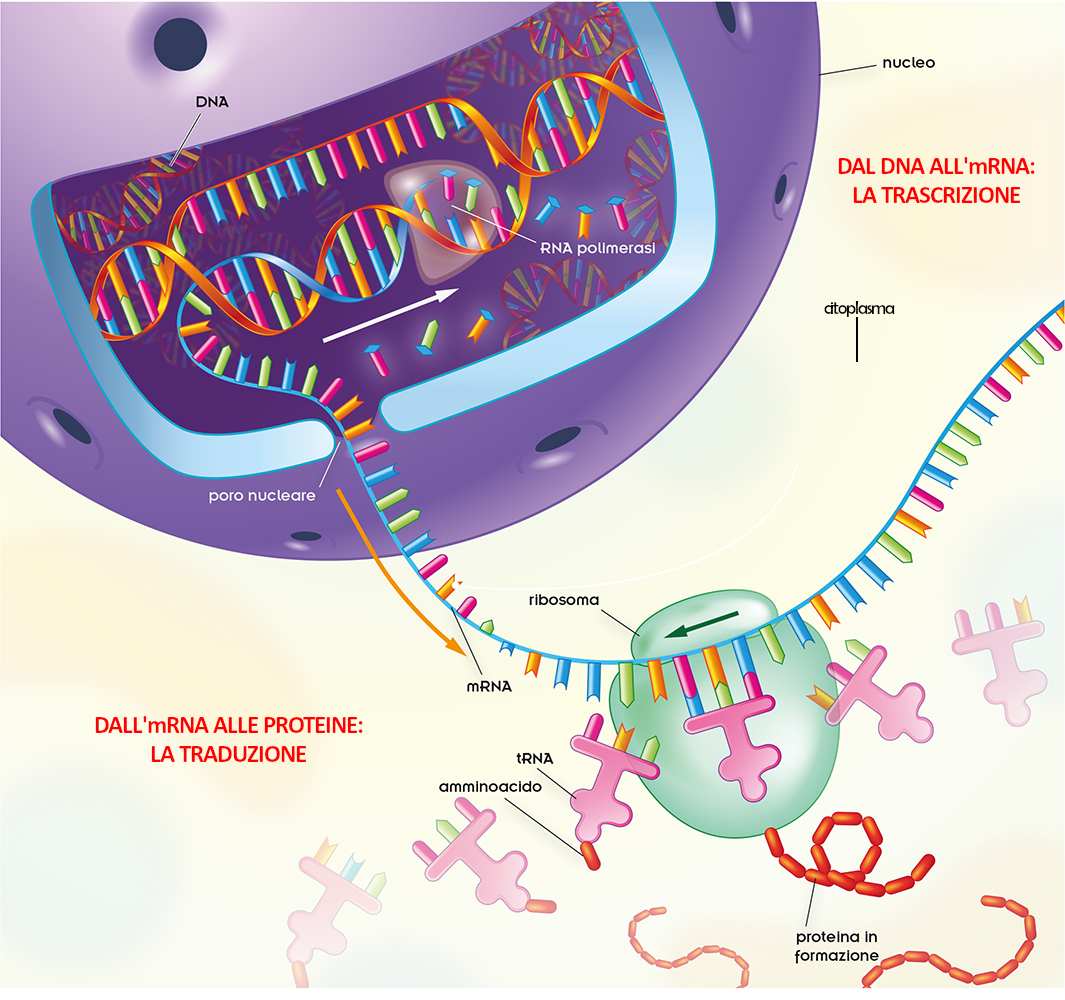
\includegraphics[width=0.9\linewidth]{images/dna_rna.jpg}
		\caption{Meccanismi di trascrizione e traduzione grazie ai quali il genotipo (l'insieme delle informazioni ereditarie di un organismo) controlla il fenotipo (le caratteristiche fisiche di un organismo) (cita
			%https://ms-mms.hubscuola.it/public/4207663/cdi-4207813/01_infog/index.html
			,
			%libro 3 anno campbell biologia
			).}
		\label{fig:dna_rna}
	\end{figure}
	
	Come già anticipato, il DNA è localizzato nel nucleo della cellula\footnote{In realtà esiste il DNA mitocondriale, un particolare tipo di DNA che contiene informazioni genetiche ereditato solo per linea materna (cita
	%libro 2 anno campbell biologia
	), che è situato all'interno dei mitocondri, organuli cellulari in cui avviene la respirazione cellulare.} ed è legato a particolari proteine che formano una struttura fibrosa chiamata cromatina, che al momento della duplicazione cellulare si addensa formando i cromosomi. Dalle considerazioni precedenti, riassunte nella \hyperref[fig:cell]{Fig. 1.11}, si comprende che il DNA occupa solo una minima parte della cellula: solamente il $2$--$3\%$ del volume cellulare è occupato da DNA. Per questo motivo arrecare danni diretti al DNA da parte di radiazione ionizzante è un evento piuttosto raro, ma non trascurabile.
	\begin{figure}[H]
		\centering
		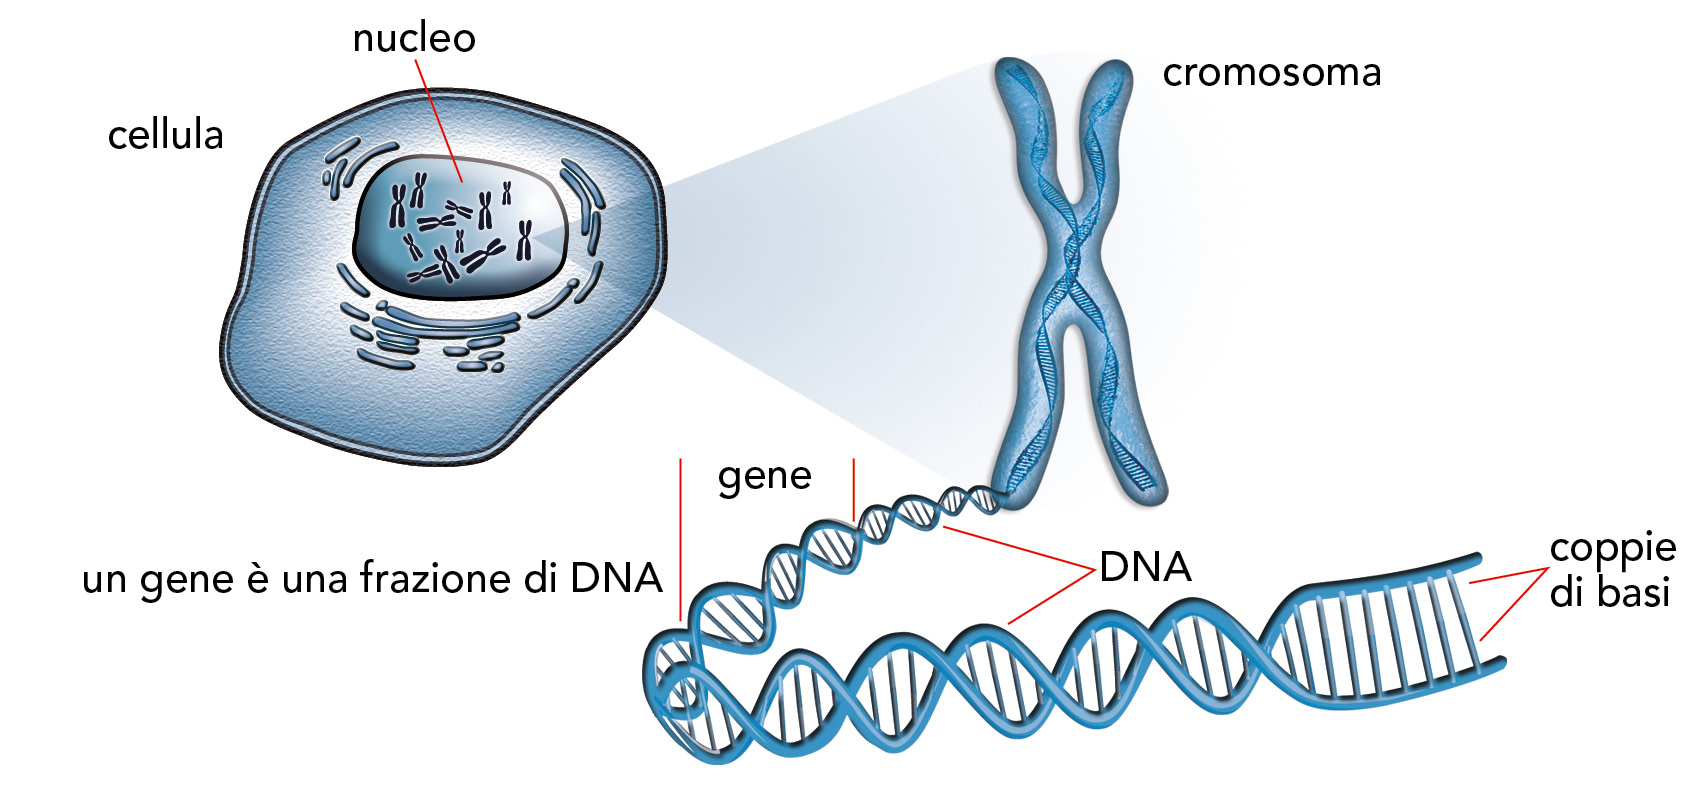
\includegraphics[width=0.9\linewidth]{images/cell.jpg}
		\caption{Particolari della struttura della cellula eucariote umana (cita
			%https://mydbook.giuntitvp.it/app/books/GIAC90_G9076812D/html/21
			).}
		\label{fig:cell}
	\end{figure}
	
	Quando la radiazione ionizzante colpisce direttamente il DNA, quest'ultimo può subire danni differenti la cui distribuzione dipende dal tipo di radiazione e dall'energia del fascio incidente. In generale, è possibile suddividere i danni in Single Strand Break (SSB) e Double Strand Breaks (DSB) in quanto nei SSB si genera la rottura di un solo filamento nucleotidico della doppia elica del DNA, mentre nei DSB si ha un danneggiamento in entrambe le catene nucleotidiche, come rappresentato in \hyperref[fig:danni_dna]{Fig. 1.12}. Grazie al meccanismo di correzione di bozze enzimi specifici come DNA polimerasi, DNA ligasi e nucleasi riconoscono i nucleotidi fuori posto e li sostituiscono (mediante un meccanismo chiamato riparazione delle anomalie di appaiamento) prima che possano portare a mutazioni genetiche.\footnote{Ricerche hanno dimostrato che difetti ereditari negli enzimi sopra citati sono associati a una forma di cancro al colon, in quanto gli errori che portano al cancro si accumulano nel DNA più velocemente (cita
	%libro campbell II anno biologia
	).} L'efficacia dei metodi di riparazione dipende dalla complessità del danno iniziale: nei SSB la catena danneggiata viene sostituita dagli enzimi osservando le informazioni della catena integra (sfruttando la complementarietà delle basi azotate), mentre nei DSB si hanno danni che non consentono una ricostruzione della doppia elica; in quest'ultimo caso la cellula potrebbe andare incontro o a morte cellulare (danno deterministico voluto in radio e adroterapia per ottenere l'eliminazione di cellule tumorali) o a carcinogenesi (danno stocastico da limitare in radio e adroterapia, la cui insorgenza è legata alle conseguenze a lungo termine dell'esposizione alla radiazione), perdendo in ambo i casi la sua capacità riproduttiva (cita
	%https://fisica.unipv.it/Eventi/Incontri-fisica-moderna/2017-12-12-Baiocco-Babini-slides.pdf
	).
	
	\begin{figure}[H]
		\centering
		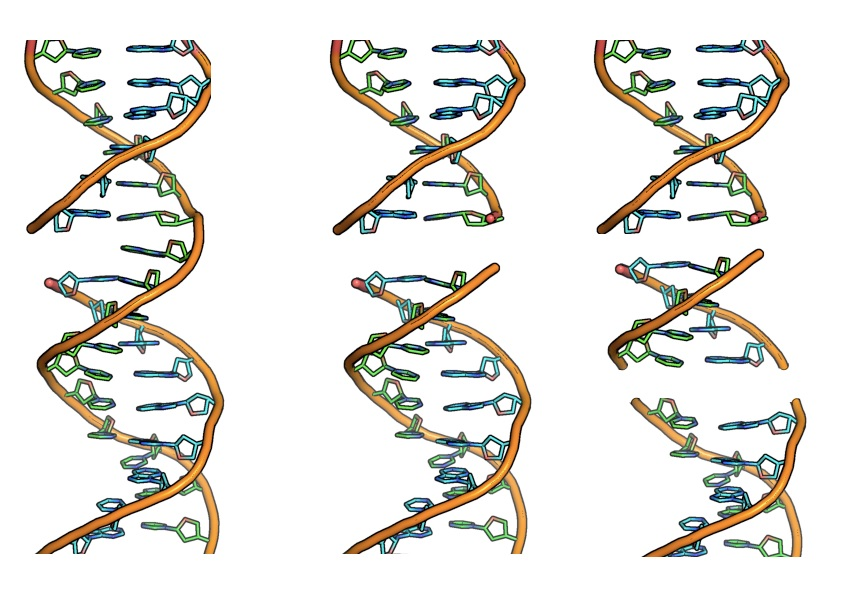
\includegraphics[width=0.9\linewidth]{images/danni_dna.jpg}
		\caption{Schematizzazione dei SSB (a sinistra), dei DSB (al centro) e di cluster di DSB (a destra) (cita
			%https://fisica.unipv.it/Eventi/Incontri-fisica-moderna/2017-12-12-Baiocco-Babini-slides.pdf
			).}
		\label{fig:danni_dna}
	\end{figure}
	
	\subsubsection{Danno indiretto}
	Per i motivi esposti nel paragrafo precedente, circa i $2/3$ dei danni cellulari si generano utilizzando radiazione ionizzante che non colpisce direttamente il DNA (cita
	%https://www.dkfz.de/en/medizinische-physik-radioonkologie/Teaching/10_LEM_Models_Carbon_RadiobiologicalModeling.pdf
	). Uno dei danni indiretti più frequenti si ha quando la radiazione colpisce l'acqua contenuta nelle cellule cancerose\footnote{Dato che il corpo umano è costituito per il $75\%$ da acqua, irradiare la cellula equivale, di fatto, a irradiare acqua.} producendo radicali liberi\footnote{I radicali liberi sono atomi neutri o molecole che possiedono un unico elettrone spaiato nel loro orbitale più esterno, caratteristica che è fonte di grande instabilità chimica; ciò rende i radicali liberi particolarmente reattivi e in grado sia di legarsi ad altri radicali sia di sottrarre elettroni a molecole vicine (cita
	%Paolo Silvestroni, Fondamenti di chimica, Bologna, Zanichelli, 1996
	).} tramite processi di radiolisi\footnote{Per radiolisi chimica si intende la scissione di uno o più legami causata da radiazioni ionizzanti (cita
	%https://goldbook.iupac.org/terms/view/R05112
	).} dell'acqua. La radiolisi dell'acqua consiste in una serie di reazioni chimiche (alcune delle quali riportate di seguito) che producono elettroni, atomi, molecole e ioni che, diffondendo, danneggiano indirettamente il DNA portando alla morte cellulare. La ionizzazione di una molecola d'acqua (\ce{H2O}) viene riassunta nella \hyperref[eq:radiolisi1]{Eq. 1.1}:
	\begin{equation}
		\ce{H2O ->[Radiazione ionizzante] H2O^{+} + e^-}
		\label{eq:radiolisi1}
	\end{equation}
	da cui si producono uno ione positivo \ce{H2O^{+}} e un elettrone \ce{e^-}. Trascorso un certo intervallo di tempo, alcuni elettroni perdono una buona parte di energia cinetica che rende possibile la cattura elettronica da parte di un'altra molecola d'acqua con conseguente formazione di uno ione negativo \ce{H2O^{-}}, come descritto nella \hyperref[eq:radiolisi2]{Eq. 1.2}:
	\begin{equation}
		\ce{H2O + e^{-} ->[Cattura elettronica] H2O^{-}}
		\label{eq:radiolisi2}
	\end{equation}
	In seguito i prodotti delle \hyperref[eq:radiolisi1]{Eq. 1.1} e \hyperref[eq:radiolisi2]{Eq. 1.2} si dissociano nei seguenti modi:
	\begin{subequations}
		\begin{align}
			\label{eq:dissociazione1}
			\ce{H2O^{+} ->[Dissociazione] H^{+} + OH^{.}}\\
			\label{eq:dissociazione2}
			\ce{H2O^{-} ->[Dissociazione] OH^{-} + H^{.}}
		\end{align}
	\end{subequations}
	i cui prodotti sono gli ioni idrogeno \ce{H^{+}} e ossidrile \ce{OH^{-}} e i radicali liberi ossidrile \ce{OH^{.}} e idrogeno \ce{H^{.}}. Tra le varie reazioni chimiche che possono avvenire successivamente, i cui reagenti sono i prodotti delle \hyperref[eq:dissociazione1]{Eq. 1.3a} e \hyperref[eq:dissociazione2]{Eq. 1.3b}, si riportano le seguenti:
	\begin{subequations}
		\begin{align}
			\label{eq:prodotto1}
			\ce{H^{.} + OH^{.} &-> H2O}\\
			\label{eq:prodotto2}
			\ce{H^{+} + OH^{-} &-> H2O}\\
			\label{eq:prodotto3}
			\ce{2OH^{.} &-> H2O2}
		\end{align}
	\end{subequations}
	Le \hyperref[eq:dissociazione1]{Eq. 1.4a} e \hyperref[eq:dissociazione2]{Eq. 1.4b} sono reazioni innocue in quanto generano molecole d'acqua mentre la \hyperref[eq:dissociazione3]{Eq. 1.4c} porta alla formazione di perossido di idrogeno (acqua ossigenata, \ce{H2O2}), una sostanza nociva per la cellula in quanto capace di modificare la struttura e le funzioni delle proteine, di mutare le basi nucleotidiche e di generare SSB nel DNA (cita
	%https://www.rndsystems.com/resources/articles/reactive-oxygen-species-ros
	). Ciò spiega il motivo per cui i danni indiretti al DNA, per mezzo della catena di radiolisi dell'acqua, portino la cellula alla morte riproduttiva (cita
	%https://www.mdpi.com/2073-4441/3/1/235
	).
	
	Il corpo umano attua una catena di meccanismi di difesa in presenza di \ce{H2O2} (e altre specie chimiche come i due radicali anione superossido \ce{O2^{-.}} e ossidrile \ce{OH^{.}}, generalmente denominate ROS (Specie Reattive all'Ossigeno)) che si attivano in maniera naturale durante le reazioni di riduzione dell'ossigeno ad acqua, da cui i mitocondri cellulari ricavano energia per il corpo umano. Il primo meccanismo di difesa è quello di disattivare il radicale \ce{O2^{-.}} tramite l'enzima superossido dismutasi (SOD), che catalizza la reazione \hyperref[eq:sod]{Eq. 1.5}:
	\begin{equation}
		\ce{2O2^{-.} + 2H^+ ->[SOD] H2O2 + O2}
		\label{eq:sod}
	\end{equation}
	in cui l'anione superossido viene trasformato in perossido di idrogeno. Successivamente, per disattivare il perossido di idrogeno, intervengono gli enzimi glutatione perossidasi e catalasi che catalizzano rispettivamente le reazioni \hyperref[eq:gsh]{Eq. 1.6a} e \hyperref[eq:catalasi]{Eq. 1.6b}:
	\begin{subequations}
		\begin{align}
			\label{eq:gsh}
			\ce{2GSH + H2O2 &->[Glutatione perossidasi] 2H2O + GSSG}\\
			\label{eq:catalasi}
			\ce{2H2O2 &->[Catalasi] 2H2O + O2}
		\end{align}
	\end{subequations}
	dove \ce{GSH} e \ce{GSSG} sono rispettivamente la forma ridotta e la forma ossidata del glutatione (il substrato\footnote{Il substrato di un enzima è un reagente specifico su cui agisce l'enzima stesso al fine di catalizzare una certa reazione chimica (cita
		%libro campbell 2 anno biologia
		).} della glutatione perossidasi) e \ce{O2} è una molecola di ossigeno.
	
	Anche le sostanze antiossidanti, come la vitamina E, consentono di catturare i radicali liberi diminuendo la loro azione dannosa. In generale, gli enzimi glutatione perossidasi e catalasi e la vitamina E hanno una concentrazione maggiore nei luoghi in cui il danno da ROS tende a essere maggiore, per esempio nei siti più ossigenati. Infatti, osservando l'\hyperref[eq:sod]{Eq. 1.5}, l'eccesso di ossigeno nei tessuti amplifica i danni dovuti all'\ce{H2O2} (si veda \hyperref[??]{oxygen enhancement ratio??}) (cita
	%https://www.rndsystems.com/resources/articles/reactive-oxygen-species-ros
	,
	%Ugo Leuzzi, Ersilia Bellocco e Davide Barreca, Biochimica della nutrizione, ISBN 978-88-08-17926-5.
	).
	
	\subsection{Grandezze dosimetriche}
	In radiobiologia la dosimetria definisce e quantifica le grandezze che descrivono l'interazione delle radiazioni ionizzanti con la materia e gli effetti biologici dell'assorbimento radiativo da parte dei tessuti del corpo umano. Nel TP dei pazienti affetti da neoplasie gli studi dosimetrici sono fondamentali in quanto consentono di misurare la quantità di radiazione necessaria all'eliminazione del tumore e i danni biologici arrecati all'organismo. Nei prossimi paragrafi si espongono le principali grandezze fisico-biologiche utilizzate in dosimetria.
	
	\subsubsection{Dose assorbita, equivalente ed efficace}
	Tra le grandezze dosimetriche caratteristiche della sorgente si trova la fluenza di particelle $\phi$, definita come il numero di particelle $dN$ (ad esempio i protoni all'interno di un fascio) per unità di superficie perpendicolare alla direzione del fascio $dS$. La fluenza è espressa nella sua forma differenziale nella \hyperref[eq:fluence]{Eq. 1.7}:
	\begin{equation}
		\phi=\frac{dN}{dA}
		\label{eq:fluence}
	\end{equation}
	Dalla fluenza di particelle è definibile la dose assorbita $D_{as}$ ossia l'energia assorbita $dE$ assorbita per unità di massa $dm$:
	\begin{equation}
		D_{as}=\frac{dE}{dm}=\frac{\left(\frac{dE}{dx}\right)\Delta x N}{\rho \Delta x A}=\phi\frac{\left(\frac{dE}{dx}\right)}{\rho}
		\label{eq:dose_as}
	\end{equation}
	dove $\left(\frac{dE}{dx}\right)$ è il potere frenante (energia persa dal fascio di particelle per unità di distanza percorsa nel mezzo irradiato), $N$ è il numero di particelle del fascio e $\rho$ è la densità di massa volumetrica del materiale irradiato. L'unità di misura della dose nel SI (Sistema Internazionale) è il Gray (Gy), tale che $1\mbox{ Gy}=1\frac{J}{kg}$. La dose assorbita è la grandezza dosimetrica per antonomasia in quanto consente di rappresentare la distribuzione della quantità di energia radiativa ricevuta dal paziente durante la terapia per unità di massa del tessuto; nonostante ciò, la $D_{as}$ non tiene conto dei diversi effetti biologici che possono essere indotti da fasci radiativi di tipo differente. Infatti, a parità di dose assorbita, il danno biologico può variare in base all'energia assorbita dal mezzo irradiato per unità di percorso (LET, si veda \hyperref[par:let]{Linear Energy Transfer}), all'Efficacia Biologica Relativa (RBE, si veda \hyperref[??]{??}) che quantifica la variabilità degli effetti biologici dovuta a radiazioni con differente LET e all'abbondanza di ossigeno nei tessuti (OER, si veda \hyperref[??]{??}) (cita
	%note dal corso di fisica biomedica a.a. 2022-2023
	). Pertanto, per includere i diversi effetti biologici dovuti a tutti i possibili tipi di radiazione $R$, si introduce la dose equivalente $D_{eq}$ definita dalla \hyperref[eq:dose_eq]{Eq. 1.9}:
	\begin{equation}
		D{eq}=\sum_{R}w_RD_{as,R}
		\label{eq:dose_eq}
	\end{equation}
	dove $D_{as,R}$ è la dose assorbita relativa alla radiazione $R$-esima e $w_R$ pondera la pericolosità della radiazione. $w_R$, denominato fattore di qualità, è il rapporto tra il danno biologico prodotto dall'assorbimento di $1\mbox{ Gy}$ della radiazione $R$ e il danno biologico prodotto da $1\mbox{ Gy}$ di raggi $\gamma$. La prima unità di misura della dose equivalente fu il rem (röntgen equivalent man), oggi sostituito dal Sievert (Sv), tale che $1\mbox{ Sv}=100\mbox{ rem}$. La $D{eq}$ è una grandezza ancora incompleta in quanto non quantifica gli effetti biologici in relazione al tipo di organo o tessuto irradiato. Pertanto si definisce la dose efficace $D_{eff}$ che comprende sia gli effetti biologici dovuti al tipo di radiazione $R$ sia quelli legati a tutti i tessuti e organi irradiati $T$. La dose efficace è definita dalla \hyperref[eq:dose_eff]{Eq. 1.10}:
	\begin{equation}
		D_{eff}=\sum_{T}w_TD_{eq}=\sum_{T}w_T\sum_{R}w_RD
		\label{eq:dose_eff}
	\end{equation}
	dove $w_T$ è un fattore di ponderazione per il tessuto $T$-esimo tale che $\sum_{T}w_T=1$, dove la somma avviene su tutti gli organi e i tessuti del corpo umano considerati sensibili all'induzione di effetti stocastici provocati dalla radiazione. In particolare, $w_T$ è maggiore per i tessuti più sensibili alla radiazione\footnote{I tessuti più sensibili alla radiazione sono quelli in cui è più facile rimuovere le cellule neoplastiche, ma sono anche i tessuti più soggetti all'insorgenza di effetti collaterali dovuti all'applicazione di radiazione ionizzante.} come quelli caratterizzati da un'elevata riproduzione cellulare, in cui l'eliminazione del cancro ha una maggiore riuscita. Anche la $D_{eff}$ si misura in Sievert, in modo che gli effetti biologici di $1\mbox{ Sv}$ di una data radiazione siano uguali a quelli di $1\mbox{ Gy}$ dei raggi $\gamma$, presi come riferimento. Si riportano alcuni valori di $w_R$ e $w_T$ in \hyperref[tab:w_factor]{Tab. 1.1}.
	
	\begin{table}[H]
		\begin{minipage}{\textwidth}
			\centering
			\begin{tabular}{ |m{0.5\textwidth}||m{0.5\textwidth}| }
				\hline
				Tipo di radiazione & $w_R$ \\
				\hline\hline
				Fotoni & 1\\
				\hline
				Elettroni e muoni & 1\\
				\hline
				Protoni e pioni carichi & 2\\
				\hline
				Particelle alfa, frammenti di fissione, nuclei pesanti & 20\\
				\hline
				Neutroni & Funzione dell'energia del neutrone\\
				\hline\hline
				Organi o tessuti & $w_T$\\
				\hline\hline
				Gonadi & 0.08 \\
				\hline
				Midollo osseo (rosso) & 0.12\\
				\hline
				Colon & 0.12\\
				\hline
				Polmone (vie respiratorie toraciche) & 0.12\\
				\hline
				Stomaco & 0.12\\
				\hline
				Mammelle & 0.12\\
				\hline
				Vescica & 0.04\\
				\hline
				Fegato & 0.04\\
				\hline
				Esofago & 0.04\\
				\hline
				Tiroide & 0.04\\
				\hline
				Pelle & 0.01\\
				\hline
				Superficie ossea & 0.01\\
				\hline
				Cervello & 0.01\\
				\hline
				Ghiandole salivari & 0.01\\
				\hline
				Rimanenti organi o tessuti\footnote{Ghiandole surrenali, regione extratoracica, vescichetta biliare, cuore, reni, linfonodi, muscolo, mucosa orale, pancreas, prostata (uomini), intestino tenue, milza, timo, utero/collo dell'utero (donne).} & 0.12\\
				\hline
			\end{tabular}
		\end{minipage}
		\caption{Tabella riassuntiva dei valori di alcuni fattori di ponderazione per la radiazione $w_R$ e per organi e tessuti $w_T$ (cita
				%pdf D.Lgs. 101-2020 in \Tesi\FOOT\Materiale
				).}
		\label{tab:w_factor}
	\end{table}
	
	\subsubsection{Linear Energy Transfer}\label{par:let}
	Il Linear Energy Transfer (LET) di una radiazione ionizzante è la quantità di energia $dE$ trasferita al materiale a causa delle collisioni per unità di distanza $dx$:
	\begin{equation}
		LET=\frac{dE_\Delta}{dx}
		\label{eq:let}
	\end{equation}
	Già nella \hyperref[eq:dose_as]{Eq. 1.8} viene utilizzato il potere frenante $\left(\frac{dE}{dx}\right)$, simile alla definizione di LET. Il motivo per cui tali termini si trattano separatamente risiede in una loro differenza: mentre il potere frenante è legato all'energia persa dal fascio di particelle nel mezzo che attraversa (per unità di distanza), il LET si riferisce all'energia assorbita dal mezzo (per unità di distanza). Nella \hyperref[eq:let]{Eq. 1.11} compare il pedice $\Delta$ in quanto nella definizione di LET si tengono conto dei trasferimenti di energia localizzati vicino alla traiettoria della particella, escludendo le ionizzazioni degli elettroni a lungo raggio più energetici la cui energia è maggiore di una soglia $\Delta$ come mostrato in \hyperref[fig:let]{Fig. 1.13}. Nel limite $\Delta\rightarrow+\infty$\footnote{Tale condizione limite non si raggiunge fisicamente, ma corrisponde al caso in cui vengono inclusi tutti i trasferimenti di energia della \hyperref[eq:let]{Eq. 1.11}, per quanto grandi possano essere.} non esisterebbero più elettroni con $E>\Delta$ in quanto l'energia persa dalla particella del fascio corrisponderebbe eguaglierebbe l'energia assorbita dal materiale (il che renderebbe equivalenti il potere frenante e il LET). Tali considerazioni consentono di ricavare la relazione che lega il potere frenante e il LET:
	\begin{equation}
		LET=\frac{dE_\Delta}{dx}-K_{E>\Delta}
		\label{eq:let&stoppingpower}
	\end{equation}
	dove $K_{E>\Delta}$ è l'energia cinetica degli elettroni che possiedono un'energia $E>\Delta$.
	
	\begin{figure}[H]
		\centering
		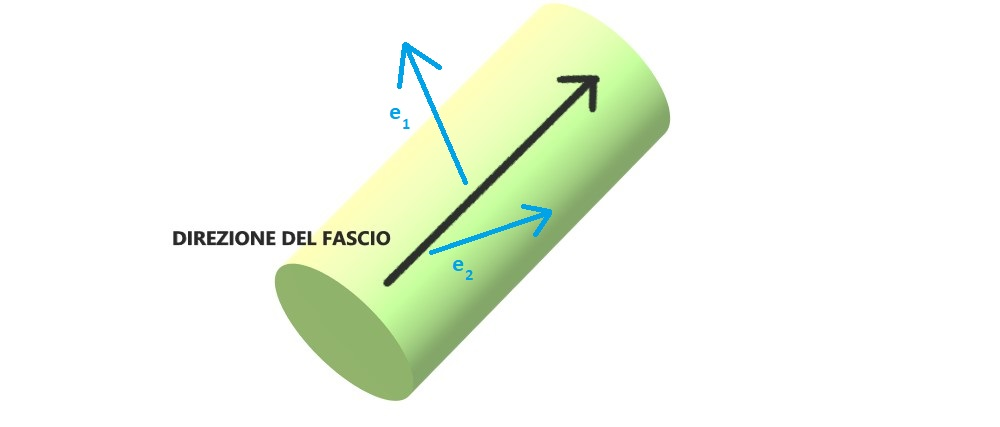
\includegraphics[width=0.9\linewidth]{images/let.jpg}
		\caption{Il cilindro schematizza la traiettoria di una particella del fascio. Gli elettroni $e_1$ ed $e_2$ possiedono energie rispettivamente $E_1>\Delta$ ed $E_2<\Delta$. Nella definizione di LET si considerano solo gli elettroni a corto raggio come $e_2$.}
		\label{fig:let}
	\end{figure}
	
	In base al LET è possibile distinguere due tipi di radiazione, quelle ad alto e basso LET. Le radiazioni a basso LET, disperdendo poca energia nei tessuti per unità di percorso, penetrano più in profondità rispetto alle radiazioni ad alto LET in quanto impiegano più tempo a esaurire l'energia che possiedono. Inoltre le radiazioni ad alto LET arrecano danni biologici maggiori ai tessuti in quanto generano eventi di ionizzazione più frequenti e ravvicinati. La \hyperref[fig:damage_let]{Fig. 1.14} mostra che le radiazioni a basso LET, per esempio raggi X o $\gamma$, inducono prevalentemente danni isolati al DNA come le SSB mentre radiazioni ad alto LET, tra cui si trovano le particelle $\alpha$ o gli ioni pesanti, generano danni più distruttivi al DNA come le DSB (cita
	%https://www.ncbi.nlm.nih.gov/pmc/articles/PMC7555951/	
	).
	
	\begin{figure}[H]
		\centering
		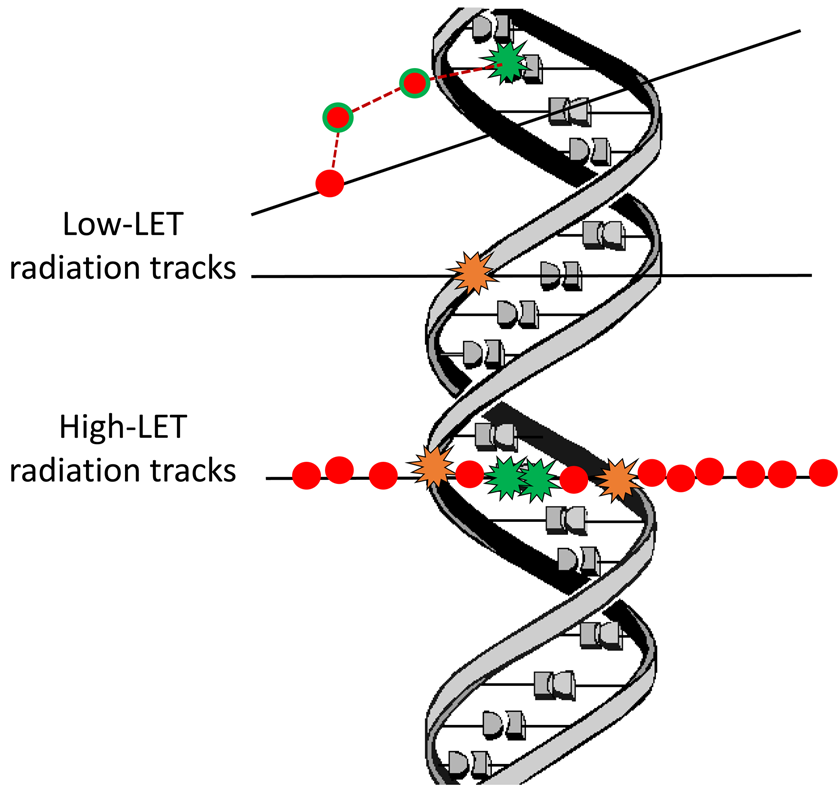
\includegraphics[width=0.9\linewidth]{images/damage_let.png}
		\caption{Danni tipici del DNA in scala nanometrica delle radiazioni a basso LET (in alto) e ad alto LET (in basso) (cita
			%https://www.cambridge.org/core/journals/expert-reviews-in-molecular-medicine/article/cell-death-mechanisms-in-head-and-neck-cancer-cells-in-response-to-low-and-highlet-radiation/5D81C15D79DA4C3B485D4367D5C7CBD3
			).}
		\label{fig:damage_let}
	\end{figure}
	
	In tabella \hyperref[tab:w_factor]{Tab. 1.2} si riassumono 
	(cita
	%
	)
	per creare danni al dna bisiogna lasciare molta energia in un piccolo spazio, che i biologi chiamano linear energy transfer (c'è una piccola differenza con de/dx). le particelle con alto let sono quelle che hanno un alto de/dx tipo i carboni, poiché fanno tante interazioni rispetto al dx.
	
	andando avanti, analizziamo una scala nanometrica. man mano che il protone entra, fa un danno ogni circa 90 nm (ma il dna è molto più piccolo quindi colpisce zone in cui non c'è il dna, almeno all'inizio); poi penetrando di più il protone fa un danno ogni 50 nm, e alla fine ogni 4 nm il che ci va bene perché il dna è dell'ordine del nm -> il carbonio, quando entra fa lo stesso effetto del protone alla fine, quindi crea danni grandi al dna sin da subito, e poi dopo fa danni "catastrofici". nella catena di ingresso la gran parte dei danni è riparabile, mentre dopo no ci sono danni permenenti, questa è una cosa importante.
	
	
	
	
	\subsubsection{RBE}
	
	\begin{table}[H]
		\centering
		\begin{tabular}{ |m{0.7\textwidth}||m{0.23\textwidth}|m{0.07\textwidth}| }
			\hline
			Tipo di radiazione & LET $\left[\mbox{keV/}\mu\mbox{m}\right]$ & RBE\\
			\hline\hline
			Raggi X ($6$--$15 \mbox{ MeV}$) & $0.3$ &	$\approx$0.8\\
			\hline
			Particella $\beta$ ($1 \mbox{ MeV}$) & 0.3 & 0.9\\
			\hline
			Protoni a energie terapiche ($150 \mbox{ MeV}$) & 0.5 & $\approx$1.1\\
			\hline
			Neutroni & $0.5$--$100$ & $1$--$2$\\
			\hline
			Particella $\alpha$ & $50$--$200$ & $5$--$10$\\
			\hline
			Ioni carbonio nella regione vicina al picco di Bragg & $40$--$90$ & $2$--$5$\\
			\hline
		\end{tabular}
		\caption{Valori approssimati di LET e RBE di alcuni tipi di radiazione (cita
			%Hasan Murshed M.D., M.S, in Fundamentals of Radiation Oncology (Third Edition), 2019
			).}
		\label{tab:let_rbe}
	\end{table}
	
	
	
	
	
	
	
	
%	l’idea di usare i protoni per il trattamento del cancro fu proposta per la prima volta nel 1946 L’adroterapia è un forma molto avanzata di radioterapia. La radioterapia, da sola o associata a chirurgia e/o a chemioterapia, migliora il controllo locale in diverse patologie tumorali. Inoltre, la natura non invasiva delle radiazioni rappresenta una valida alternativa per quei tumori non aggredibili chirurgicamente perché localizzati in sedi anatomiche complicate da organi vitali o deputati a funzioni la cui asportazione sarebbe troppo invalidante per il paziente.
	
%	La forza dell’adroterapia è nelle proprietà fisiche e radiobiologiche uniche delle particelle cariche (adroni): esse possono penetrare nei tessuti con poca diffusione e depositare la massima energia appena prima di fermarsi. Ciò consente di definire in modo molto preciso la region da irradiare. La caratteristica forma a picco del deposito di energia è chiamata picco di Bragg ed è diventata il simbolo dell’adroterapia.

% dire che FOOT L'esperimento FOOT unisce laboratori giapponesi, tedeschi e italiani al ne di raccogliere dati fondamentali per migliorare la conoscenza delle interazioni tra i fasci adronici e il materiale

% NOTA: end point è il goal che voglio raggiungere. tutti i tumori vicini a organi a rischio hanno percnetuali di soluzione molto molto elevate rispetto alla radioterapia.
	
	
	
	
			
	\addcontentsline{toc}{chapter}{Conclusioni (TBD)}
	\chapter*{Conclusioni (TBD)}
		Let's cite! Einstein's journal paper \cite{einstein} and Dirac's book \cite{dirac} are physics-related items.
	\newpage	
	\printbibliography[
		heading=bibintoc,
		title={Bibliografia}
		]
		 	
\end{document}

